% Pass options BEFORE aastex loads hyperref
\PassOptionsToPackage{
  colorlinks=true,
  citecolor=blue,
  linkcolor=black,
  urlcolor=blue
}{hyperref}

\documentclass[preprint]{aastex701}

\usepackage{amsmath}

\shorttitle{Lomb--Scargle Place Cell Detection}
\shortauthors{Groner}

% AASTeX loads natbib automatically
\setcitestyle{numbers,square,super,comma,sort&compress}

\begin{document}

\title{Lomb--Scargle Periodogram for Place Cell Detection}

\author{Jacob Groner}
\affiliation{Cornell University}
\email{jrg349@cornell.edu} % put your real email here

\begin{abstract}
    A place cell is a neuron found in the hippocampus whose activity depends on the animal's location. When recording from thousands of neurons simultaneously, it becomes necessary to develop an algorithmic method for detecting place cells. In this project, I develop a novel technique for detecting place cells and use it to evaluate neural behavior in a foraging task. The technique involves transforming the data to the spatial frequency domain via a Lomb-Scargle periodogram and performing a signal to noise ratio (SNR) calculation at target frequency.

    
\end{abstract}

\section{Introduction}

\subsection{Hippocampus and Place Cells}

Ever since the study of the lesion patient H.M., the hippocampus has been a brain region implicated in memory formation. \citep{scoville1957hm} Further study into the activity of hippocampal neurons reveal that some of these neurons track spatial position. These neurons, termed place cells, exhibit tuning curves centered on specific spatial locations. \citep{okeefe1971spatialmap} As an animal travels through its environment, different place cells become sequentially active. Over time, synaptic connections between sequentially activated cells are strengthened, while others are weakened. This leads to a population of cells whose connective structure matches the structure of the environment, with each location in the environment being represented by a unique subpopulation of neurons. This internal world model is referred to as the brain's cognitive map, \citep{okeefe1978cognitivemap} and is the basis for how an animal stores a memory. By activating patterns of place cells without actually moving, an animal can use this internal world model for planning and inspiration.

\subsection{Traditional Place Cell Detection Methods}
With the advancements of modern neuroscience, it has become possible to record from thousands of neurons simultaneously, making manual inspection of the entire dataset infeasible. To solve this problem, some methods have been developed to identify cells whose tuning curves have certain good properties. The first step in most methods is spatial binning. The physical space on which the animal is able to travel gets split into many small regions. Next, the data points get sorted based on what region the animal was in at the time when the neural activity was recorded. Then, for each region, the mean activity is computed. 

Following spatial binning, different strategies can be used to give the cell a score on how likely a cell is to be a place cell. Some common methods include the Peak method, \citep{fournier2020distance} Stability method, \citep{oleary2019stability} Combination method, \citep{dombeck2010imaging} and Information method. \citep{ziv2013longterm} For example, the Peak method compares the cell's peak activity (maximum over all bins) to the peak activity after temporal shuffling of the bins. If the real peak lies in the 99th percentile of many different shuffles, then it is classified as a place cell. While the Peak method is a standard for place cell classification across neuroscience research, \citep{grijseels2021choice} it is highly sensitive to spatial binning and uneven occupancy. \citep{Grieves2023RateMapQuant} For this reason, this project considers an alternative strategy for place cell detection which relies on frequency rather than spatial binning.

\subsection{Fourier Transform}

The Fourier transform is a mathematical equation which represents a time series signal in terms of its frequency components. 
\begin{equation}
\hat{f}(\omega) = \int_{-\infty}^{\infty} f(t)\, e^{-i \omega t}\, dt,
\end{equation}
Where $t$ denotes time and $\omega$ the corresponding angular frequency. \citep{bracewell2000fourier} Euler's formula demonstrates that the Fourier transform works by splitting the signal into an infinite sum of sinusoids of varying frequencies. The result is a complex-valued function which encodes both amplitude and phase information. Often, it is sufficient to discard the phase information and work solely with the frequency information. This is accomplished by taking the magnitude of the Fourier transform, denoted as the power spectrum. \citep{bracewell2000fourier}
\begin{equation}
P(\omega) = \lvert \hat{f}(\omega) \rvert^2
\end{equation}
A phase-invariant quantification of how the variance of a signal is distributed provides a robust framework for analyzing time series data. However, computing the pure Fourier transform for actual data is impossible because there is a discrete sampling frequency and a finite observation window. Instead, the Discrete Fourier Transform (DFT) can approximate the Fourier transform by sacrificing resolution. \citep{bracewell2000fourier}
\begin{equation}
X_k = \sum_{n=0}^{N-1} x_n \, e^{-2\pi i k n / N},
\qquad k = 0, 1, \ldots, N-1.
\end{equation}
Where $x_n = f(n\Delta t)$ denotes the discretely sampled signal, and $X_k$ represents the corresponding Fourier coefficients evaluated at discrete frequency indices $k$. The Fast Fourier Transform (FFT) algorithm recursively evaluates the Fourier transform as a sum of smaller Fourier transforms. The FFT algorithm enables computation of the DFT and corresponding power spectrum in $\mathcal{O}(N \log N)$ time, where $N$ is the number of data points. \citep{bergland1969guided} 

\subsection{Lomb--Scargle Periodogram}

One key condition for Fourier transforms is that the data is uniformly sampled. Without this condition, $x_n \neq f(n\Delta t)$ and the DFT no longer corresponds to the continuous Fourier transform. Additionally, the recursive definition used in FFT falls apart when some samples are missing, making the efficiency gains of FFT inapplicable. Moreover, with nonuniform sampling, there is no single well-defined Nyquist frequency, meaning that accounting for aliasing and spectral leakage in the power spectrum becomes much more difficult. The Lomb--Scargle algorithm presents an alternative way to directly approximate the power spectrum of a signal with non-uniform sampling. \citep{lomb1976}

The Lomb--Scargle algorithm takes in time-series data and a range of frequencies. For each frequency, it computes a normalized power value. The power values for all the frequencies gives an approximation of the power spectrum.\citep{scargle1982} To compute a power value for an angular frequency $\omega$, the first step is to fit the data to the following sinusoidal function using Least Squares Regression.
\begin{equation}
\hat{y}_\omega(t) = A \cos(\omega t) + B \sin(\omega t).
\end{equation}
Next, the chi squared error of $\hat{y}_\omega$ is computed. Equivalently, the error of the null hypothesis, $y=0$, is computed. (normalize data to have zero mean) Following this, the power is given by the normalized difference between the error of the least squares fit and the error of the null hypothesis.
\begin{equation}
P(\omega)
=
\frac{\chi^2_0 - \chi^2(\omega)}{\chi^2_0},
\end{equation}
Where $\chi^2_0$ is the chi squared error of the null hypothesis and $\chi^2(\omega)$ is the chi squared error of $\hat{y}_\omega$. Thus, the power computed by the Lomb--Scargle Periodogram can be interpreted as the relative variance accounted for by a least squares fit of a sinusoidal of particular frequency. Notably, when sampling is uniform, this method is equivalent to the classical Fourier periodogram. \citep{scargle1982}

\section{Methods}

\subsection{Data Collection}

Calcium imaging was performed using a transgenic mouse line expressing the genetically encoded calcium indicator GCaMP in hippocampal neurons. Mice were anesthetized while a small region of cortex was aspirated in order to install a glass imaging window. A headbar was additionally installed to secure the mouse to the virtual reality rig. Once the mice recovered from surgery (approximately one week), they were headfixed on a treadmill surrounded by three screens. A water port extended towards their mouth to deliver water rewards when appropriate. First, the mice were trained to run in the dark  and received a water reward after traveling a certain distance. Once the mice had passed a certain threshold in running speed and duration (took approximately one week), the screens were turned on, displaying a linear corridor. From this point on, when the mouse ran forward on the treadmill, the projected walls moved past the mouse, giving the illusion that the mouse was traveling down the corridor. The wall patterns were homogenous except for three distinct cue patterns which repeated in order. Over time, the mouse learned that if they stopped near the third cue they would receive a water reward. The mice performed one hour running sessions every day for up to two weeks. During running, a 2-photon mesoscope recorded the activity of over one thousand individual neurons. Each day, micro adjustments to the scope were made in order to continue tracking the same population of cells. An image registration step verified that the individual cells lined up across sessions.  

This data collection effort described above is part of a larger project which is currently unpublished. The experimental methods and motivations behind this larger project were adapted from \citet{sun2025osm}. Due to the scope of this paper as a class assignment, further details about the experimental methods are omitted. Consistent with the scope of this work, analyses were restricted to three sessions recorded from a single mouse. This mouse had a single one hour session every day, and the sessions selected were Day 1, Day 7, and Day 14. 2795 cells were tracked across all three sessions.

\begin{figure}[ht!]
\centering

% Top row: two images side-by-side
\begin{minipage}[t]{0.48\textwidth}
\vspace{0pt}
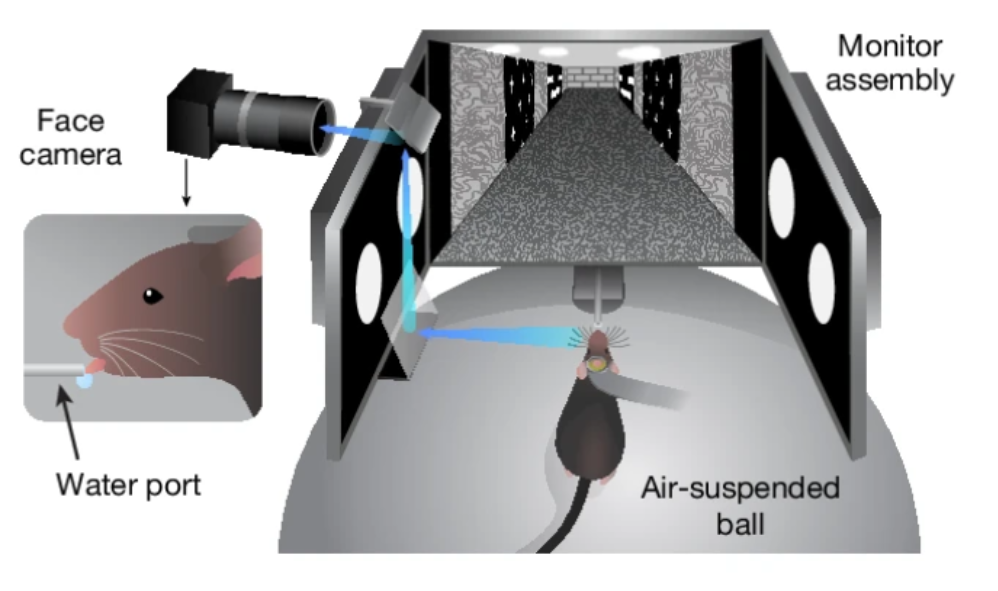
\includegraphics[width=\textwidth]{vr_setup.png}
\end{minipage}\hfill
\begin{minipage}[t]{0.48\textwidth}
\vspace{0pt}
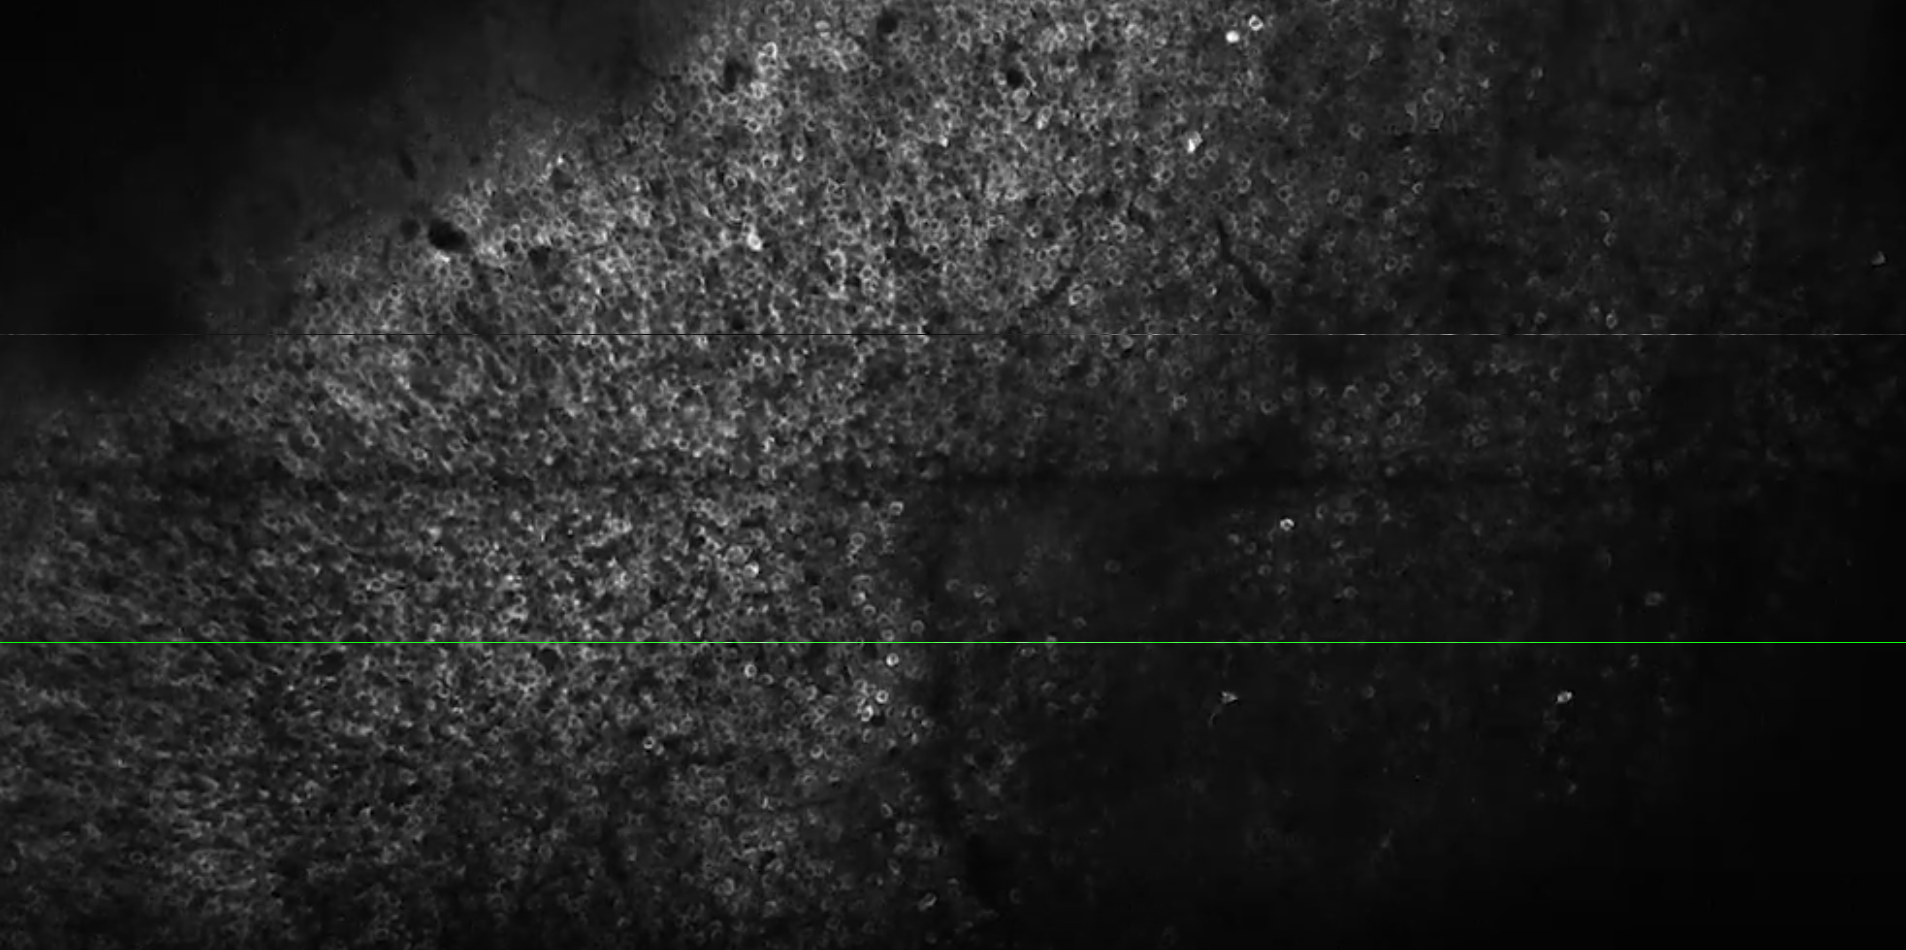
\includegraphics[width=\textwidth]{cell_image.png}
\end{minipage}

\vspace{0.02\textwidth}

% Bottom row: one full-width image
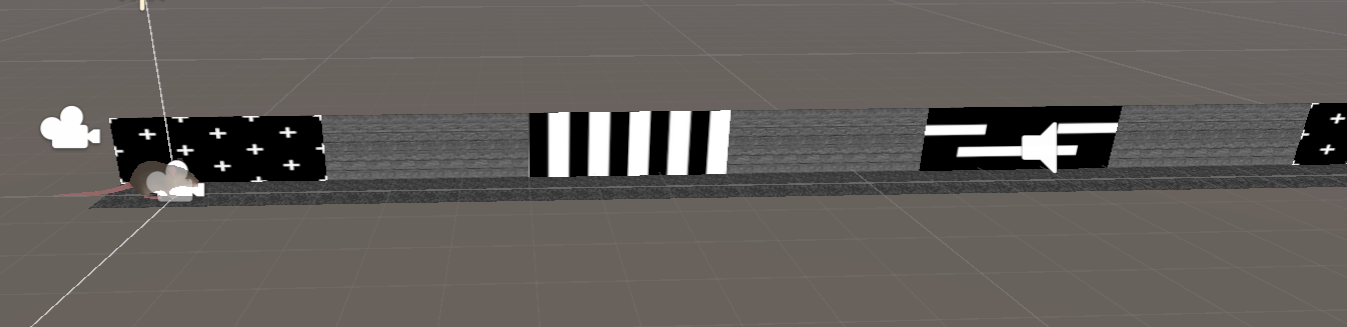
\includegraphics[width=0.98\textwidth]{task_structure.png}

\caption{
\textbf{Experimental task and recording setup.}
(\textit{Top left}) Virtual reality treadmill setup used for head-fixed calcium imaging.
(\textit{Top right}) Example two-photon field of view showing segmented hippocampal neurons.
(\textit{Bottom}) Virtual reality environment showing three unique cues.
Each cue spans $30\,\mathrm{cm}$ and cues are separated by $30\,\mathrm{cm}$,
resulting in a repeating track segment of $180\,\mathrm{cm}$.
}

\label{fig:task_overview}
\end{figure}


\subsection{Place Cell Identification}

Of the 2795 cells tracked, the goal was to identify which cells' firing patterns corresponded to the mouse's position in the virtual reality track. A cell with the property of being active when the mouse is near a specific cue and inactive when the mouse is away from that cue will likely be a neuron essential for learning the task structure and correctly navigating to the water reward. The goal was accomplished by taking advantage of the task structure. Since the task is composed of a repeating 180 cm segment, each of the three cues repeats every 180 cm. Thus, the spatial frequency of any position in the track is 1/180 cm$^{-1}$. Similarly, a cell tuned to any location in the track will necessarily spike once every 180 cm, since the mouse has to physically walk along the treadmill to move the virtual reality environment. To identify such cells, the neuronal activity was transformed to the spatial frequency domain with a focus on the 1/180 cm$^{-1}$ frequency band. 

The inspiration for this approach came from power spectral analyses used in pulsar timing experiments.  Just as long time-series measurements of pulse arrival times are converted into the frequency domain to detect weak periodic or quasi-periodic signals,\citep{arzoumanian2018nanograv11yr} the power at specific spatial frequencies (like once-per-lap for place cells) indicates meaningful structure in neural data. In both cases, the frequency content of the observed signal, rather than raw time series alone, provides a robust way to detect patterns against noise. 

In order to evaluate the power of the 1/180 cm$^{-1}$ frequency band, the power spectrum needed to be computed with respect to position, not time. The sampling rate for the neural data was a uniform 10 Hz. However, the mouse did not move at a constant speed during the entire session. Instead, it would perform bouts of sprinting followed by stops when it was drinking the water reward or getting tired. Thus, the sampling rate was nonuniform with respect to position. Thus, instead of computing the power spectrum directly from the DFT, a Lomb--Scargle Periodogram with respect to position was used to approximate the power spectrum despite a nonuniform sampling rate. 

For SNR-based ranking, Lomb--Scargle periodograms were evaluated on a fixed spatial-frequency grid spanning
$0$--$0.05~\mathrm{cm}^{-1}$ with 1{,}000 uniformly spaced frequencies
($\Delta f \approx 5 \times 10^{-5}~\mathrm{cm}^{-1}$).
This grid includes the DC component, the fundamental track frequency
($1/180~\mathrm{cm}^{-1}$), and several higher harmonics, while excluding higher
spatial frequencies dominated by noise.
For visualization of selected cells, a higher-resolution grid
(50{,}000 frequencies spanning $0$--$0.1~\mathrm{cm}^{-1}$) was used.


\subsection{Ranking Cells by Signal to Noise Ratio}

While much insight was gained by manually inspecting the periodograms, automatic place cell detection required that the periodogram be converted into a single value which represented the likelihood that the recorded neuron was a place cell. Then, simply taking the n cells with the highest likelihood would give the best n cells to study deeply how their activity changes as the mouse learns to complete the task. The likelihood estimate used was the Signal to Noise Ratio (SNR).

Suppose the periodogram is evaluated at \( N \) discrete frequencies
\( \{ f_k \}\)

\begin{equation}
\mathrm{SNR}
=
\frac{
P\!\left( f_{\mathrm{place}} \right) - \mu
}{
\sigma
}
\end{equation}

Where \( P(f_k) \) is the Lomb--Scargle Power evaluated at the spatial frequency \( f_k \), and \( f_{\mathrm{place}} = \tfrac{1}{180}\,\mathrm{cm}^{-1} \), the spatial frequency of the track. Mean and standard deviation were computed excluding the DC component (\( k = 0 \)).

\begin{equation}
\mu
=
\frac{1}{N-1}
\sum_{k=1}^{N-1}
P(f_k)
\end{equation}

\begin{equation}
\sigma
=
\sqrt{
\frac{1}{N-1}
\sum_{k=1}^{N-1}
\left( P(f_k) - \mu \right)^2
}
\end{equation}

The cells were ranked by their SNR. The SNR measures how many standard deviations the power at the target frequency is above the mean background power. Thus, the SNR is directly proportional to the likelihood that a cell is a place cell.

\subsection{Traditional Spatial Binning}

Once place cells were identified using the novel method, the traditional spatial binning approach was used to determine which cue each identified neuron was responding to. First, For each data point, the relative position within the track segment was computed by taking the total distance traveled modulo \(180\,\mathrm{cm}\). The track was then separated into 100 bins, such that each bin had a width of \(1.8\,\mathrm{cm}\). Each data point was assigned to its corresponding spatial bin based on this relative position. Finally, the mean value of the neural activity within each bin was computed. Plotting the bin positions against their corresponding mean values produced a one-dimensional place field for each cell.

\section{Results}

\subsection{Characteristic Place Cell Periodogram Structure}

\begin{figure}
    \centering
    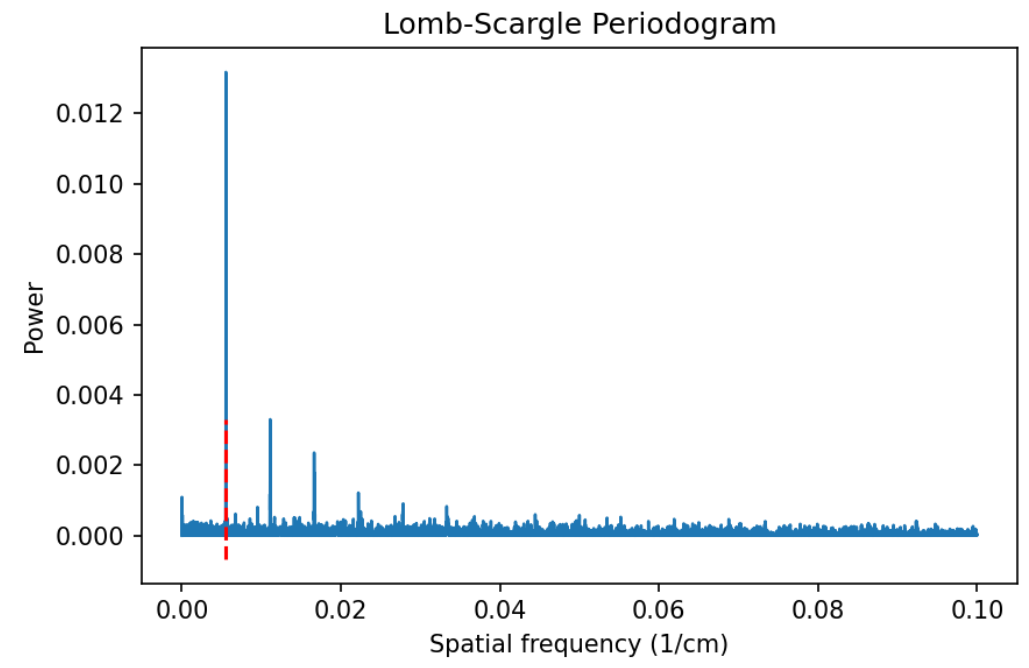
\includegraphics[width=1\linewidth]{c1566s14per.png}
    \caption{Periodogram for cell 1566's activity on Day 14. The red dashed line indicates the target frequency of \(1/180 \mathrm{cm}^{-1}\)}. 
    \label{fig:best_cell_per}
\end{figure}

In general, the SNR rankings allowed for identification of place cells. One such highly ranked cell is shown in Figure~\ref{fig:best_cell_per}. This cell had a SNR of 30.4, the third highest SNR of all cells for Day 14. The periodogram has maximum power exactly at the target frequency of \(1/180 \mathrm{cm}^{-1}\). Furthermore, the noise is dominated by periodic peaks at multiples of this fundamental frequency. These harmonics decrease in power as the multiples get larger. Another feature noticeable from the plot is the DC component, which demonstrates that the cell activity is not zero mean. This is simply because the cell activity was measured by fluorescence in a calcium indicator, which is represented as a positive number proportional to the cell's firing frequency. It is okay that the DC component is not removed from the power spectrum since the SNR calculation explicitly ignores the DC component. Nearly every cell's periodogram had harmonics which were multiples of the target frequency \(1/180 \mathrm{cm}^{-1}\). 


The harmonics suggest that while the cellular activity is highly tuned to the track position, the activity of the cell is not sinusoidal. This makes sense because the canonical definition of a place cell is a cell that bursts at a target location and has little to no activity anywhere else. For a signal which has a periodic pulse waveform, harmonics like this are expected. To verify this analysis, we consider the binned activity of the cell, shown in figure Figure~\ref{fig:best_cell_rm}. This cell clearly exhibits the bursting activity expected by a place cell. Specifically, this cell begins bursting once the mouse sees the second cue, and is pretty much inactive everywhere else in the track. This cell is not an outlier: the other top ranked cells express similar looking place cells, though centered at different track locations. The automatic identification of this cell based on SNR shows that the Lomb--Scargle Periodogram is a useful tool for classifying place cells. 

\begin{figure}
    \centering
    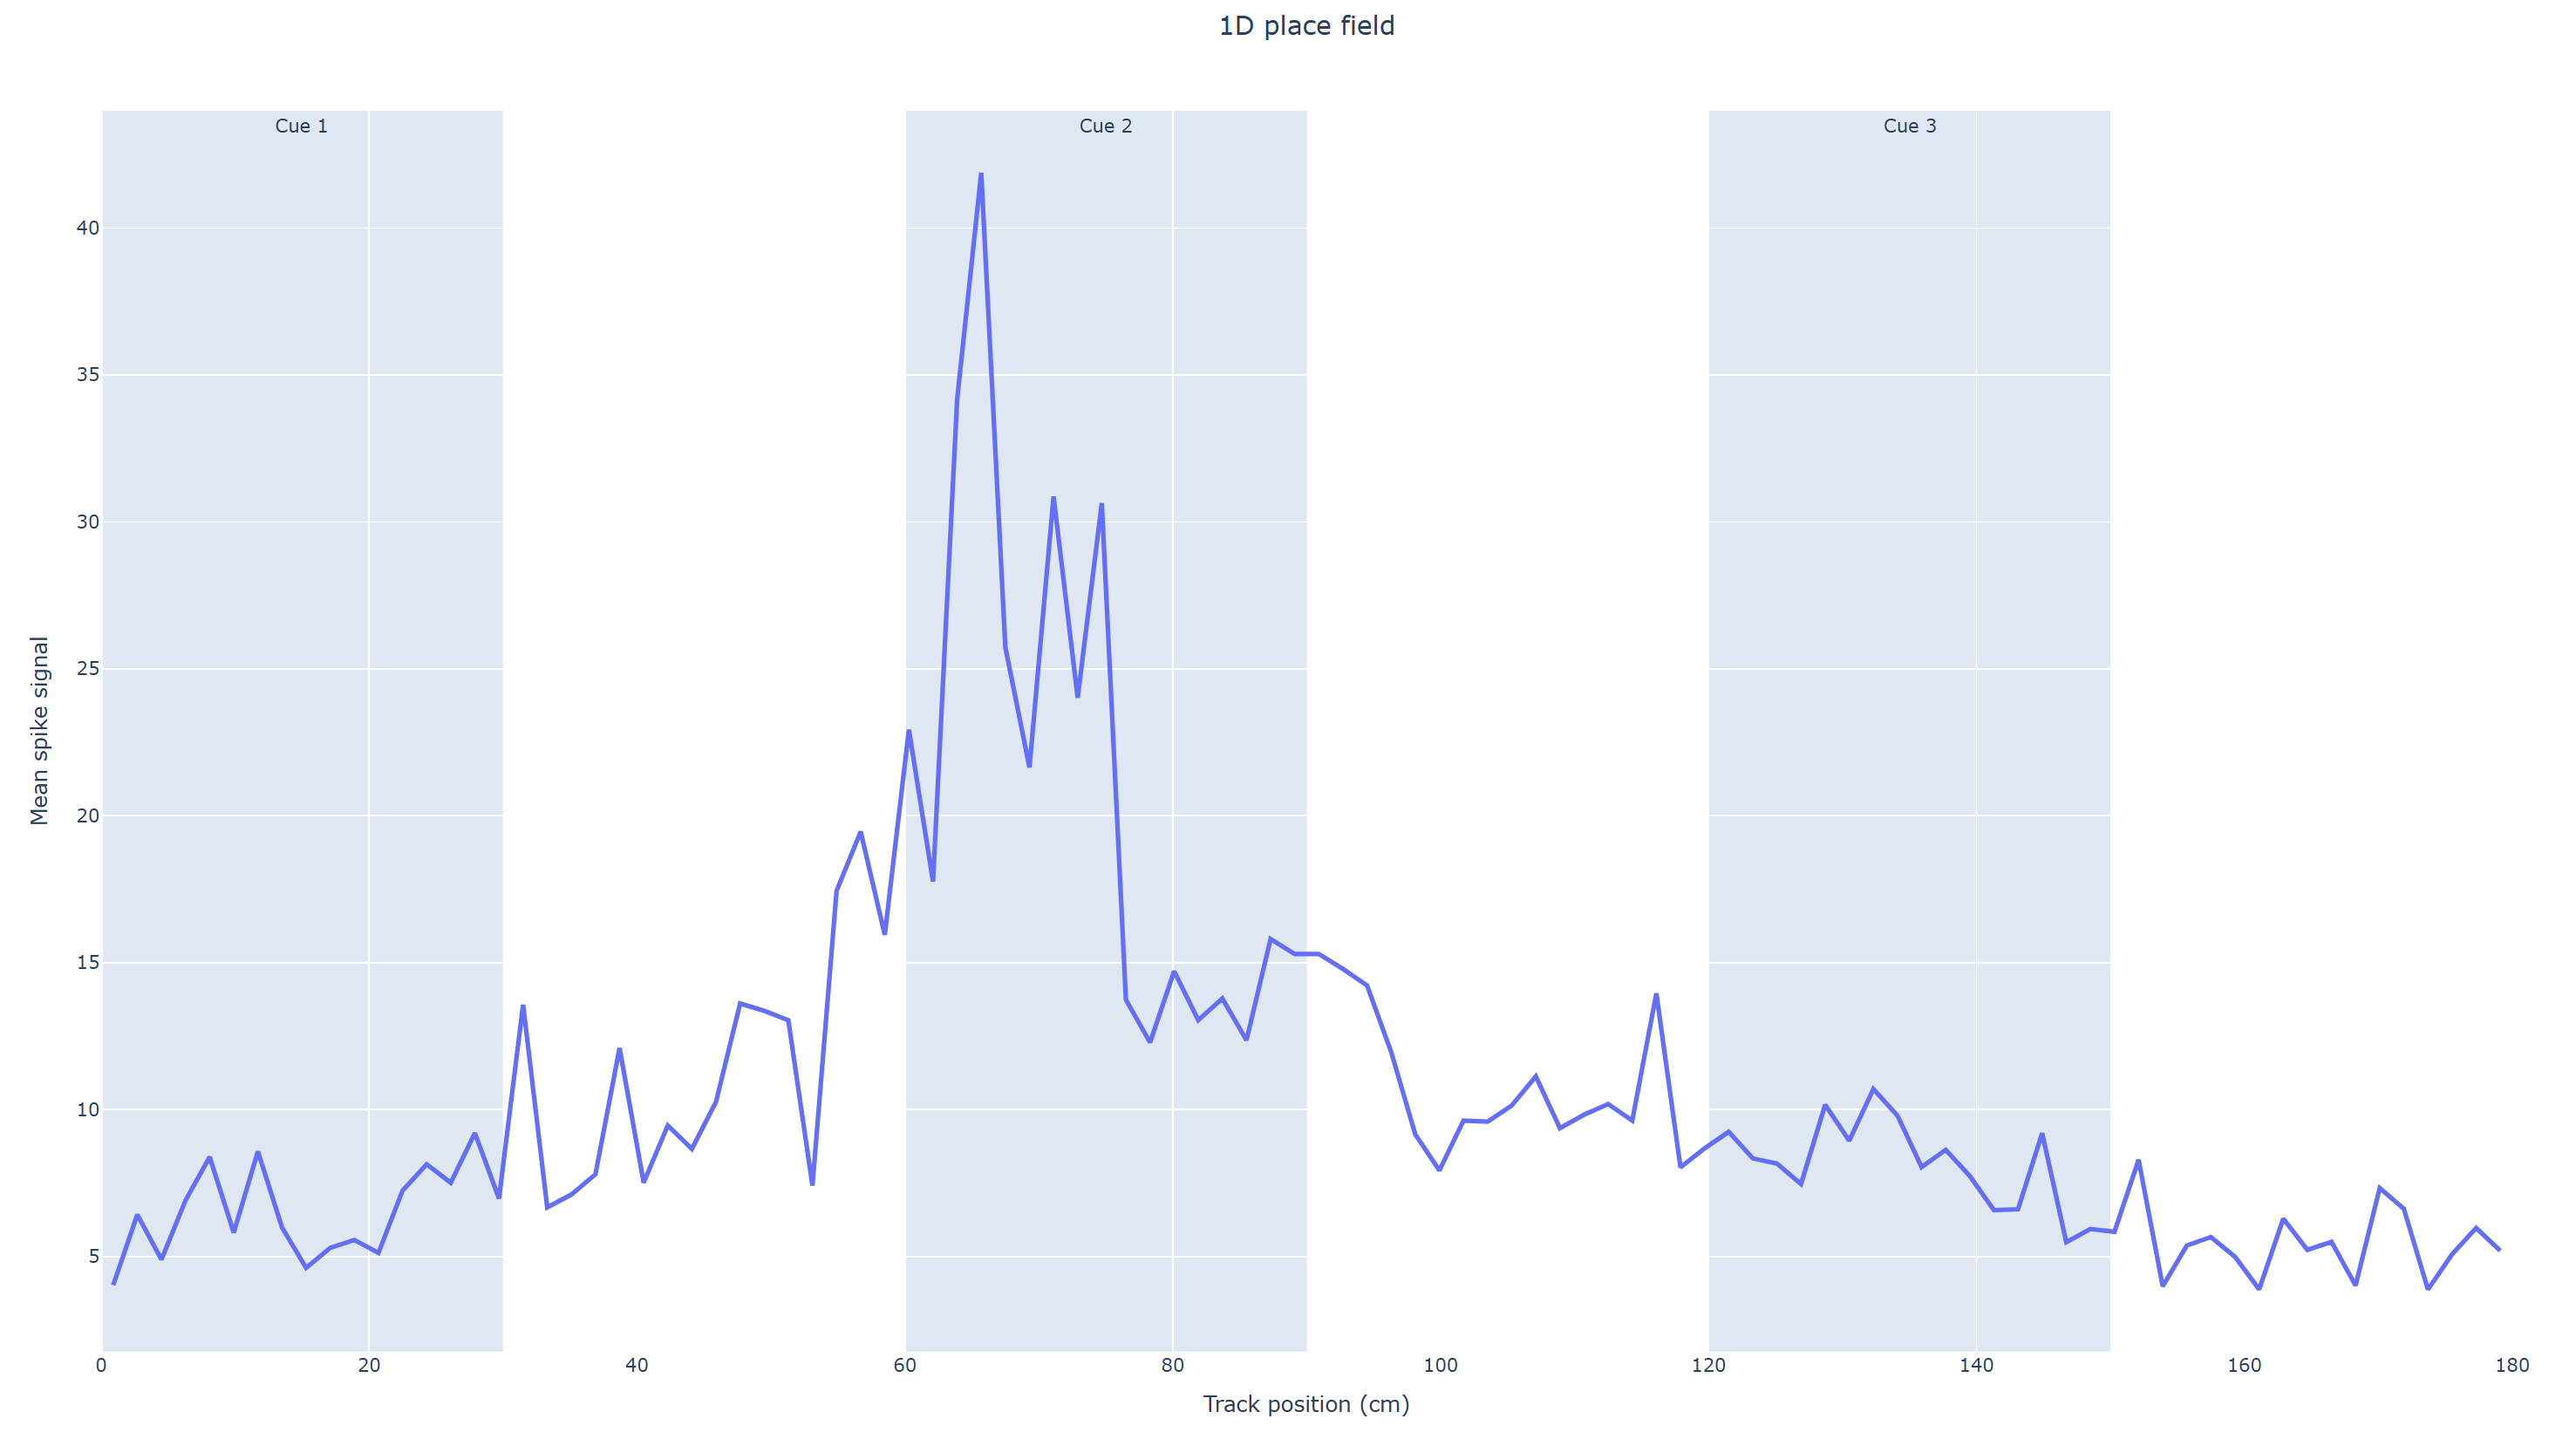
\includegraphics[width=1\linewidth]{c1566s14rm.png}
    \caption{Rate map for cell 1566's activity on Day 14. The x-axis is track position relative to the first cue. The y-axis is the normalized fluorescence, which is proportional to the cell's firing rate.} 
    \label{fig:best_cell_rm}
\end{figure}

\subsection{Periodogram of a Low SNR Cell}

Next, we compare the periodogram of cells with high SNR to the periodogram of cells with low SNR. Figure~\ref{fig:worst_cell} shows the cell with the worst SNR for Day 14, -0.980233. For reference, on Day 14, the mean SNR was 11.805940, with a standard deviation of 8.208296. The periodogram for this cell is dominated by noise, and it is not a clear peak at the fundamental frequency \(1/180 \mathrm{cm}^{-1}\). This sort of periodogram suggests that no signal is present at the selected spatial frequency. This implies that the cell is not a place cell. This can be verified by plotting the rate map for the cell, also shown in Figure~\ref{fig:worst_cell}. The rate map lacks any clear peak, and fires highly at many different locations. This suggests that the activity of the cell is not tuned to any specific location in the track. 

\begin{figure}[ht!]
\centering

\begin{minipage}[t]{0.49\textwidth}
\vspace{0pt}
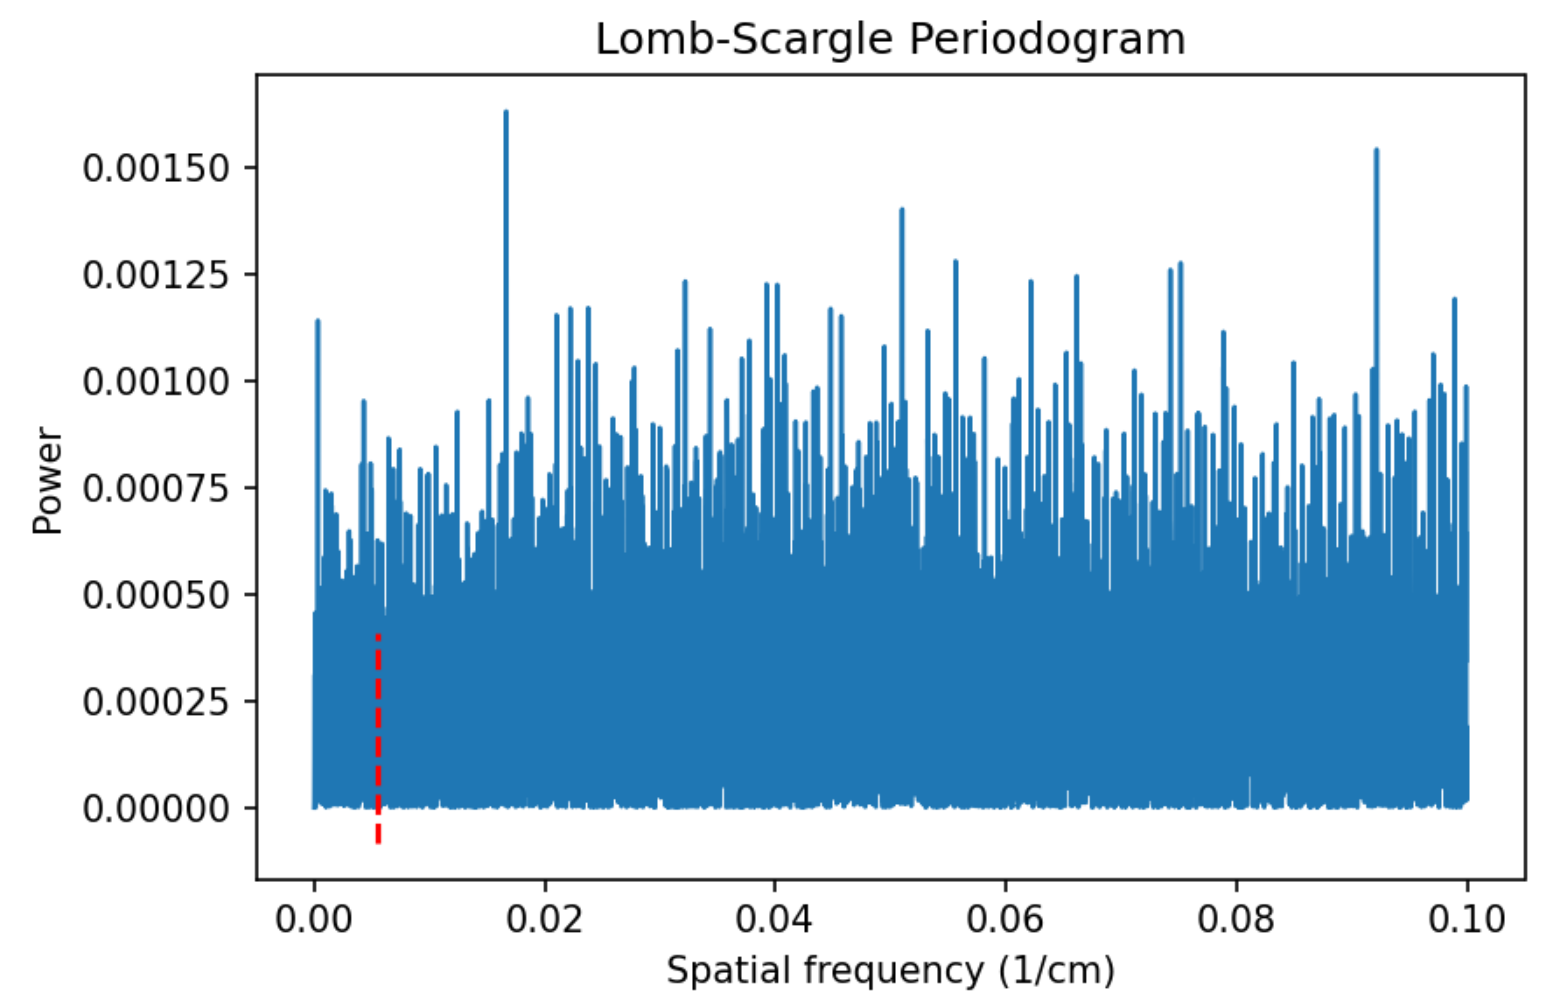
\includegraphics[width=\linewidth]{c2749s14per.png}
\end{minipage}\hfill
\begin{minipage}[t]{0.49\textwidth}
\vspace{0pt}
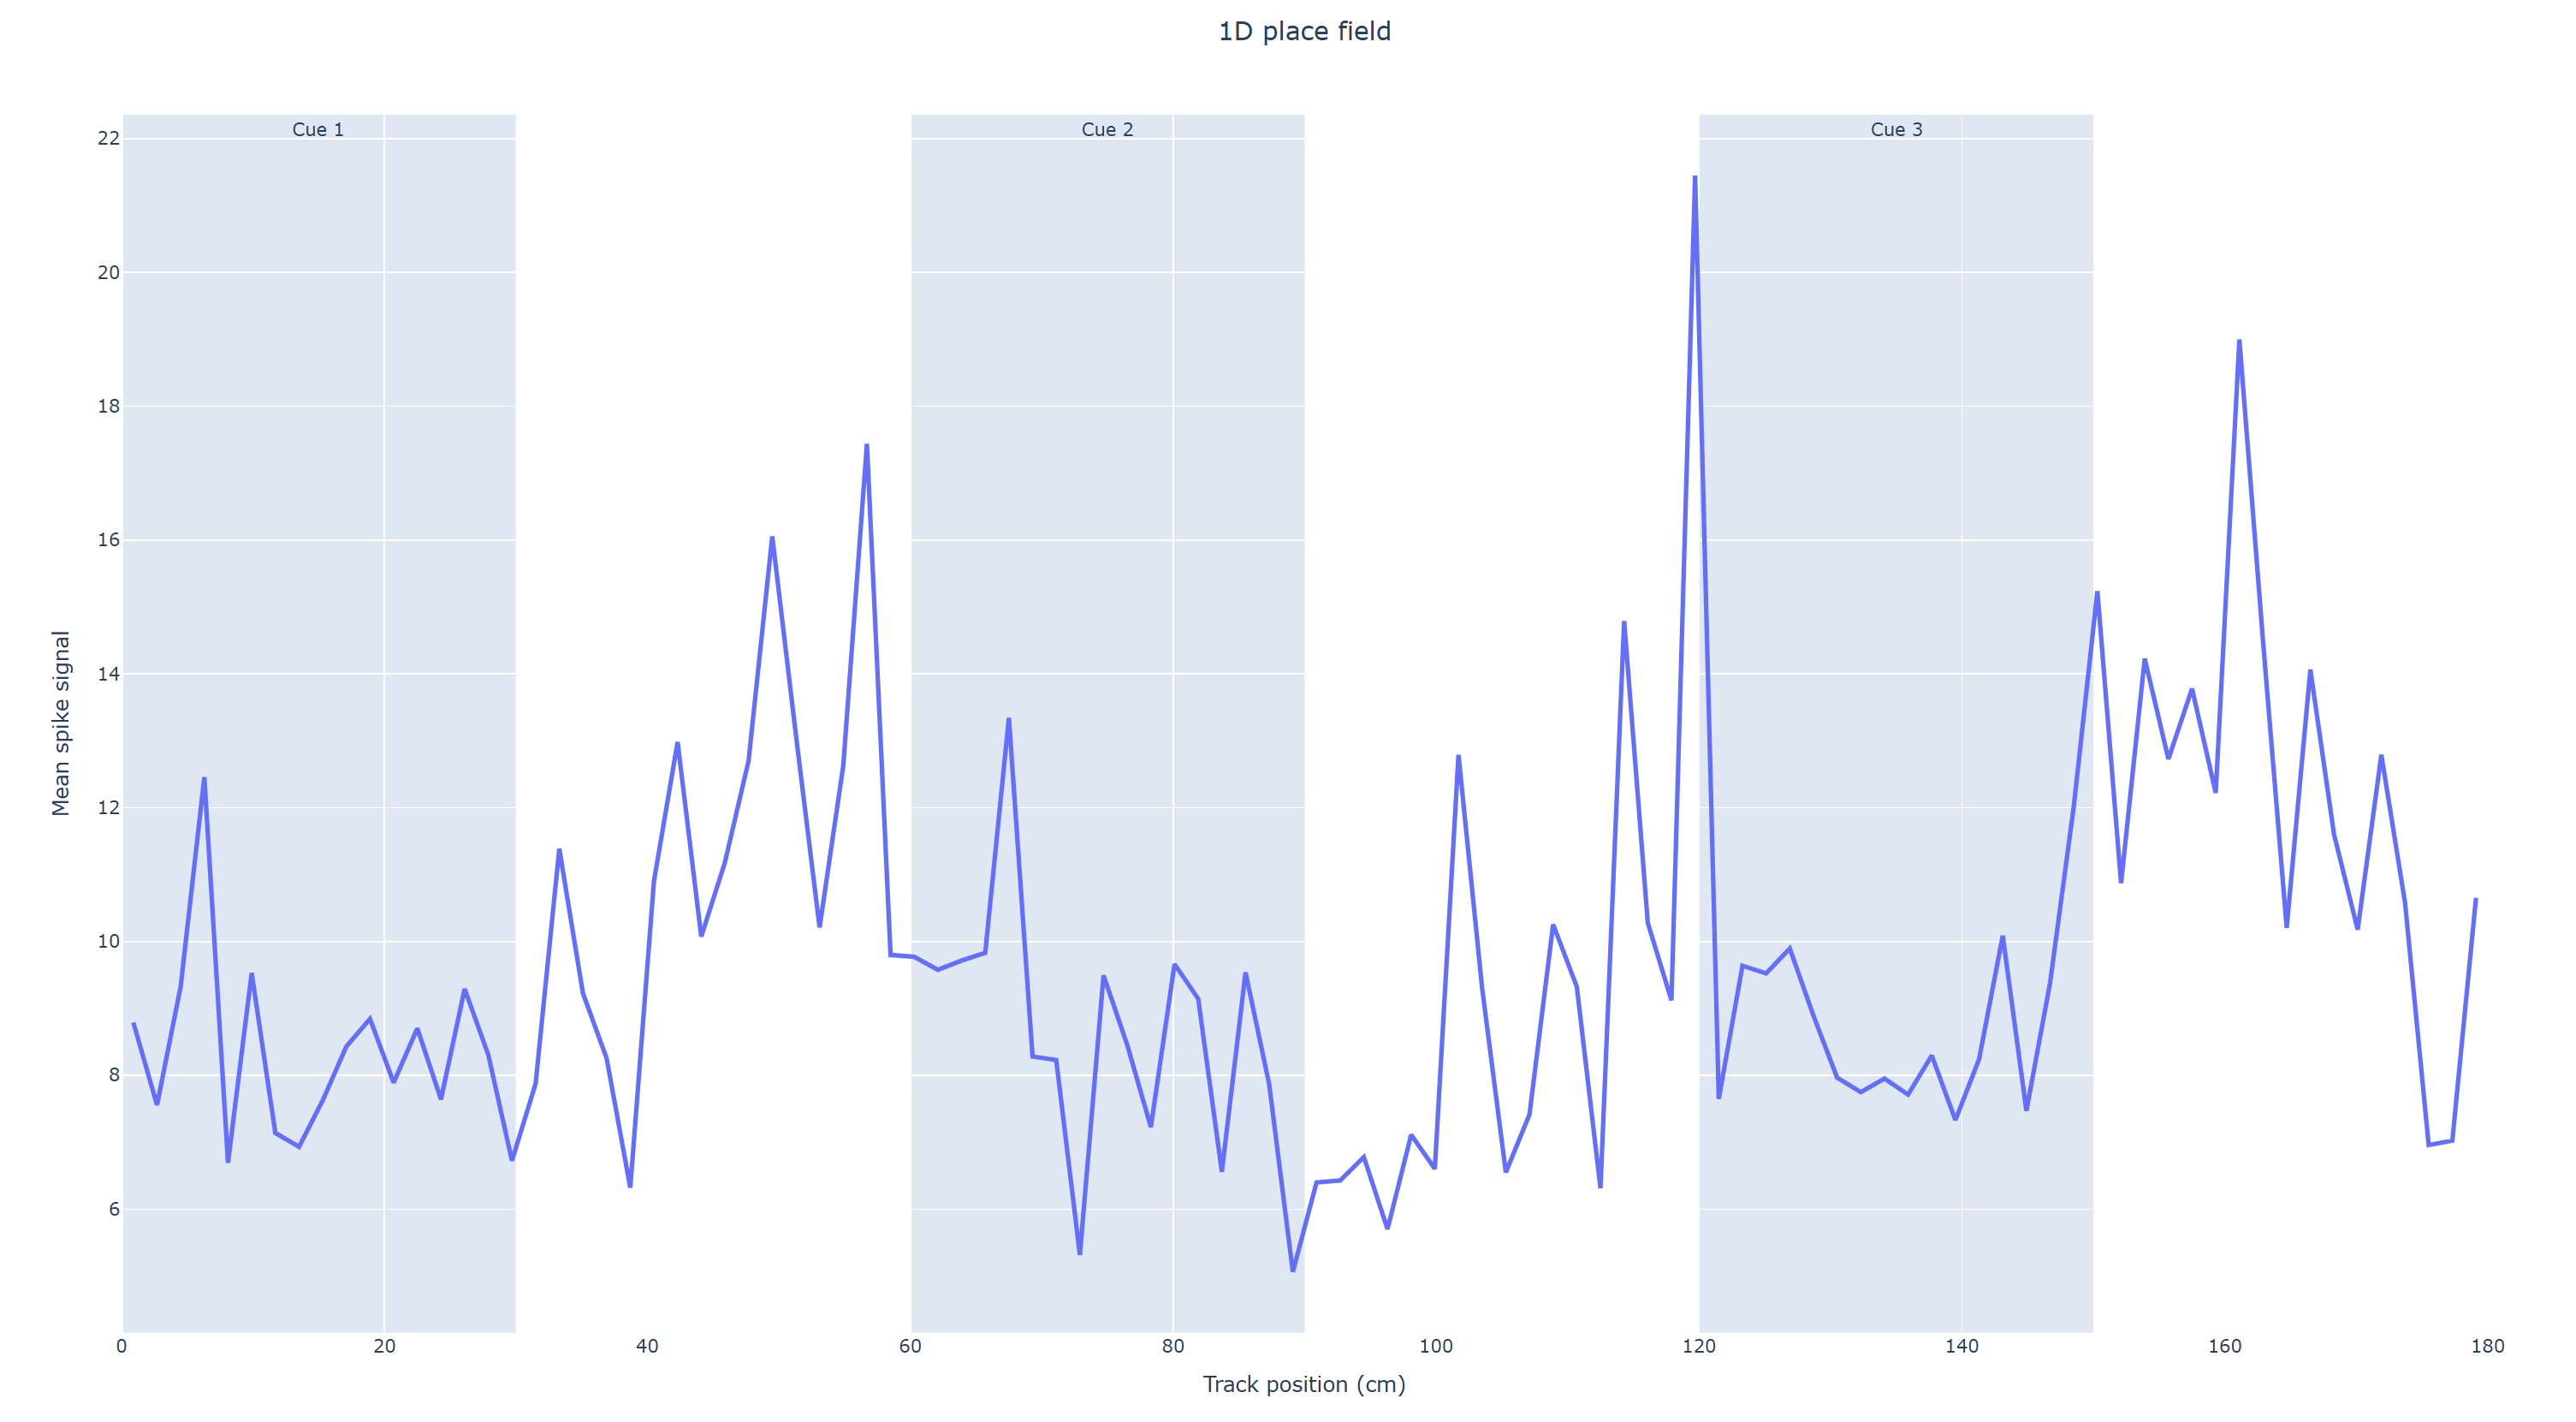
\includegraphics[width=\linewidth]{c2749s14rm.png}
\end{minipage}

\caption{
(\textit{Left}) Lomb--Scargle periodogram for cell 1566. The red dashed line indicates the target spatial frequency \(1/180~\mathrm{cm}^{-1}\).
(\textit{Right}) Rate map for cell 1566. The x-axis is track position relative to the first cue, and the y-axis is normalized fluorescence (proportional to firing rate).
}
\label{fig:worst_cell}
\end{figure}

\subsection{SNR Changes Across Sessions}

\begin{figure}[ht!]
\centering
\setlength{\tabcolsep}{10pt}
\renewcommand{\arraystretch}{1.25}
\begin{tabular}{lcc}
\hline
\textbf{Session} & \textbf{Mean SNR} & \textbf{Std. dev.} \\
\hline
Day 1  & 6.476 & 5.960 \\
Day 7  & 9.159 & 8.025 \\
Day 14 & 11.806 & 8.208 \\
\hline
\end{tabular}
\caption{ Mean and standard deviation of Lomb--Scargle SNR values across all tracked cells for each session.}
\label{fig:snr_table}
\end{figure}


Since the same cells were tracked over the course of multiple weeks, the changes in periodogram shape and time between sessions were inspected. Note that the day 1 activity was recorded during the first time the mouse ever attempted the task. In comparison, by day 14, the mouse was well acclimated to the task and consistently navigated to the reward location. Thus, it is likely that the learning process is reflected by the change in activity of task relevant place cells. One possible way that the mouse brain improved its performance on the task was by recruiting more hippocampal place cells to respond to track locations. By recruiting more cells, the representation can become more fine grained, allowing the mouse to disambiguate between different cues more effectively. Figure~\ref{fig:snr_table} shows the mean SNR across all cells for each of the three days. Between each of the three sessions, there is an increase in the mean SNR. This directly supports the claim that improving at a specific task involves recruiting more cells to tune their firing to features of that environment. The identification of place cells based on the strength of the fundamental frequency provides a direct metric for the amount of task relevant place cells. Thus, the increase in mean SNR indicates learning over time. 

\begin{figure}[ht!]
\centering

% -------- Row 1: Day 1 --------
\begin{minipage}[t]{0.48\textwidth}
\vspace{0pt}
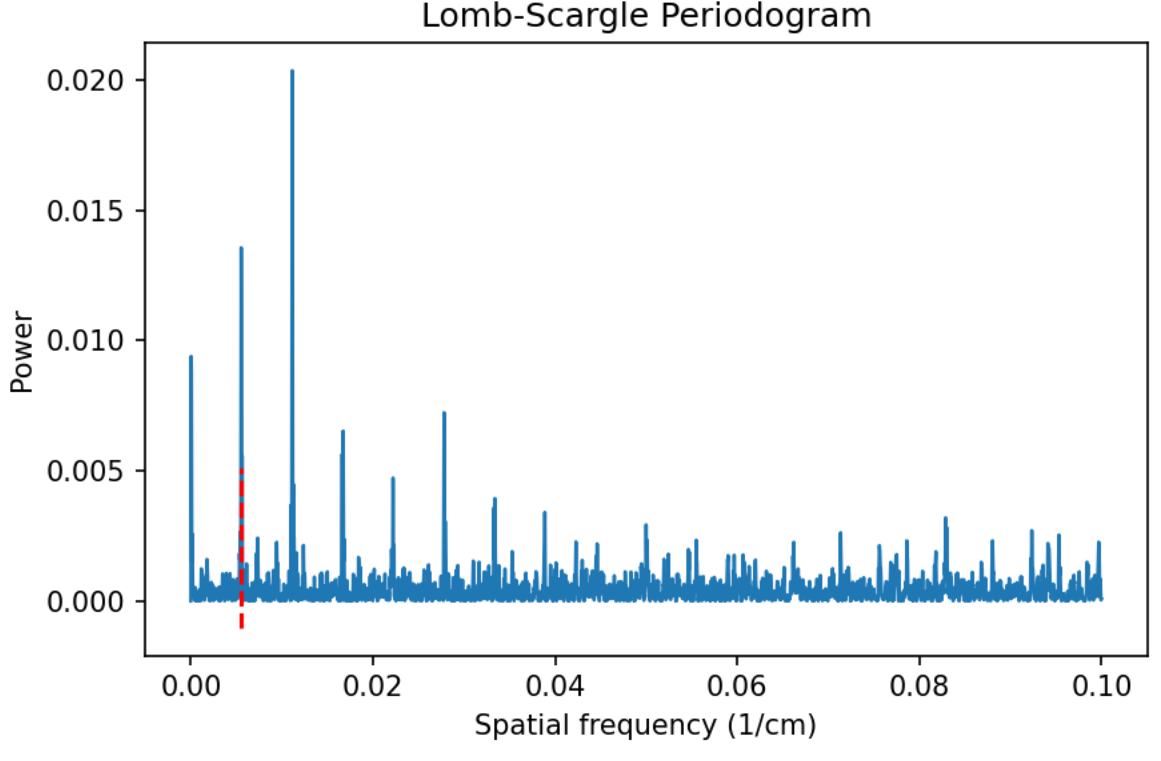
\includegraphics[width=\linewidth]{c2621_day1_per.png}
\end{minipage}\hfill
\begin{minipage}[t]{0.48\textwidth}
\vspace{0pt}
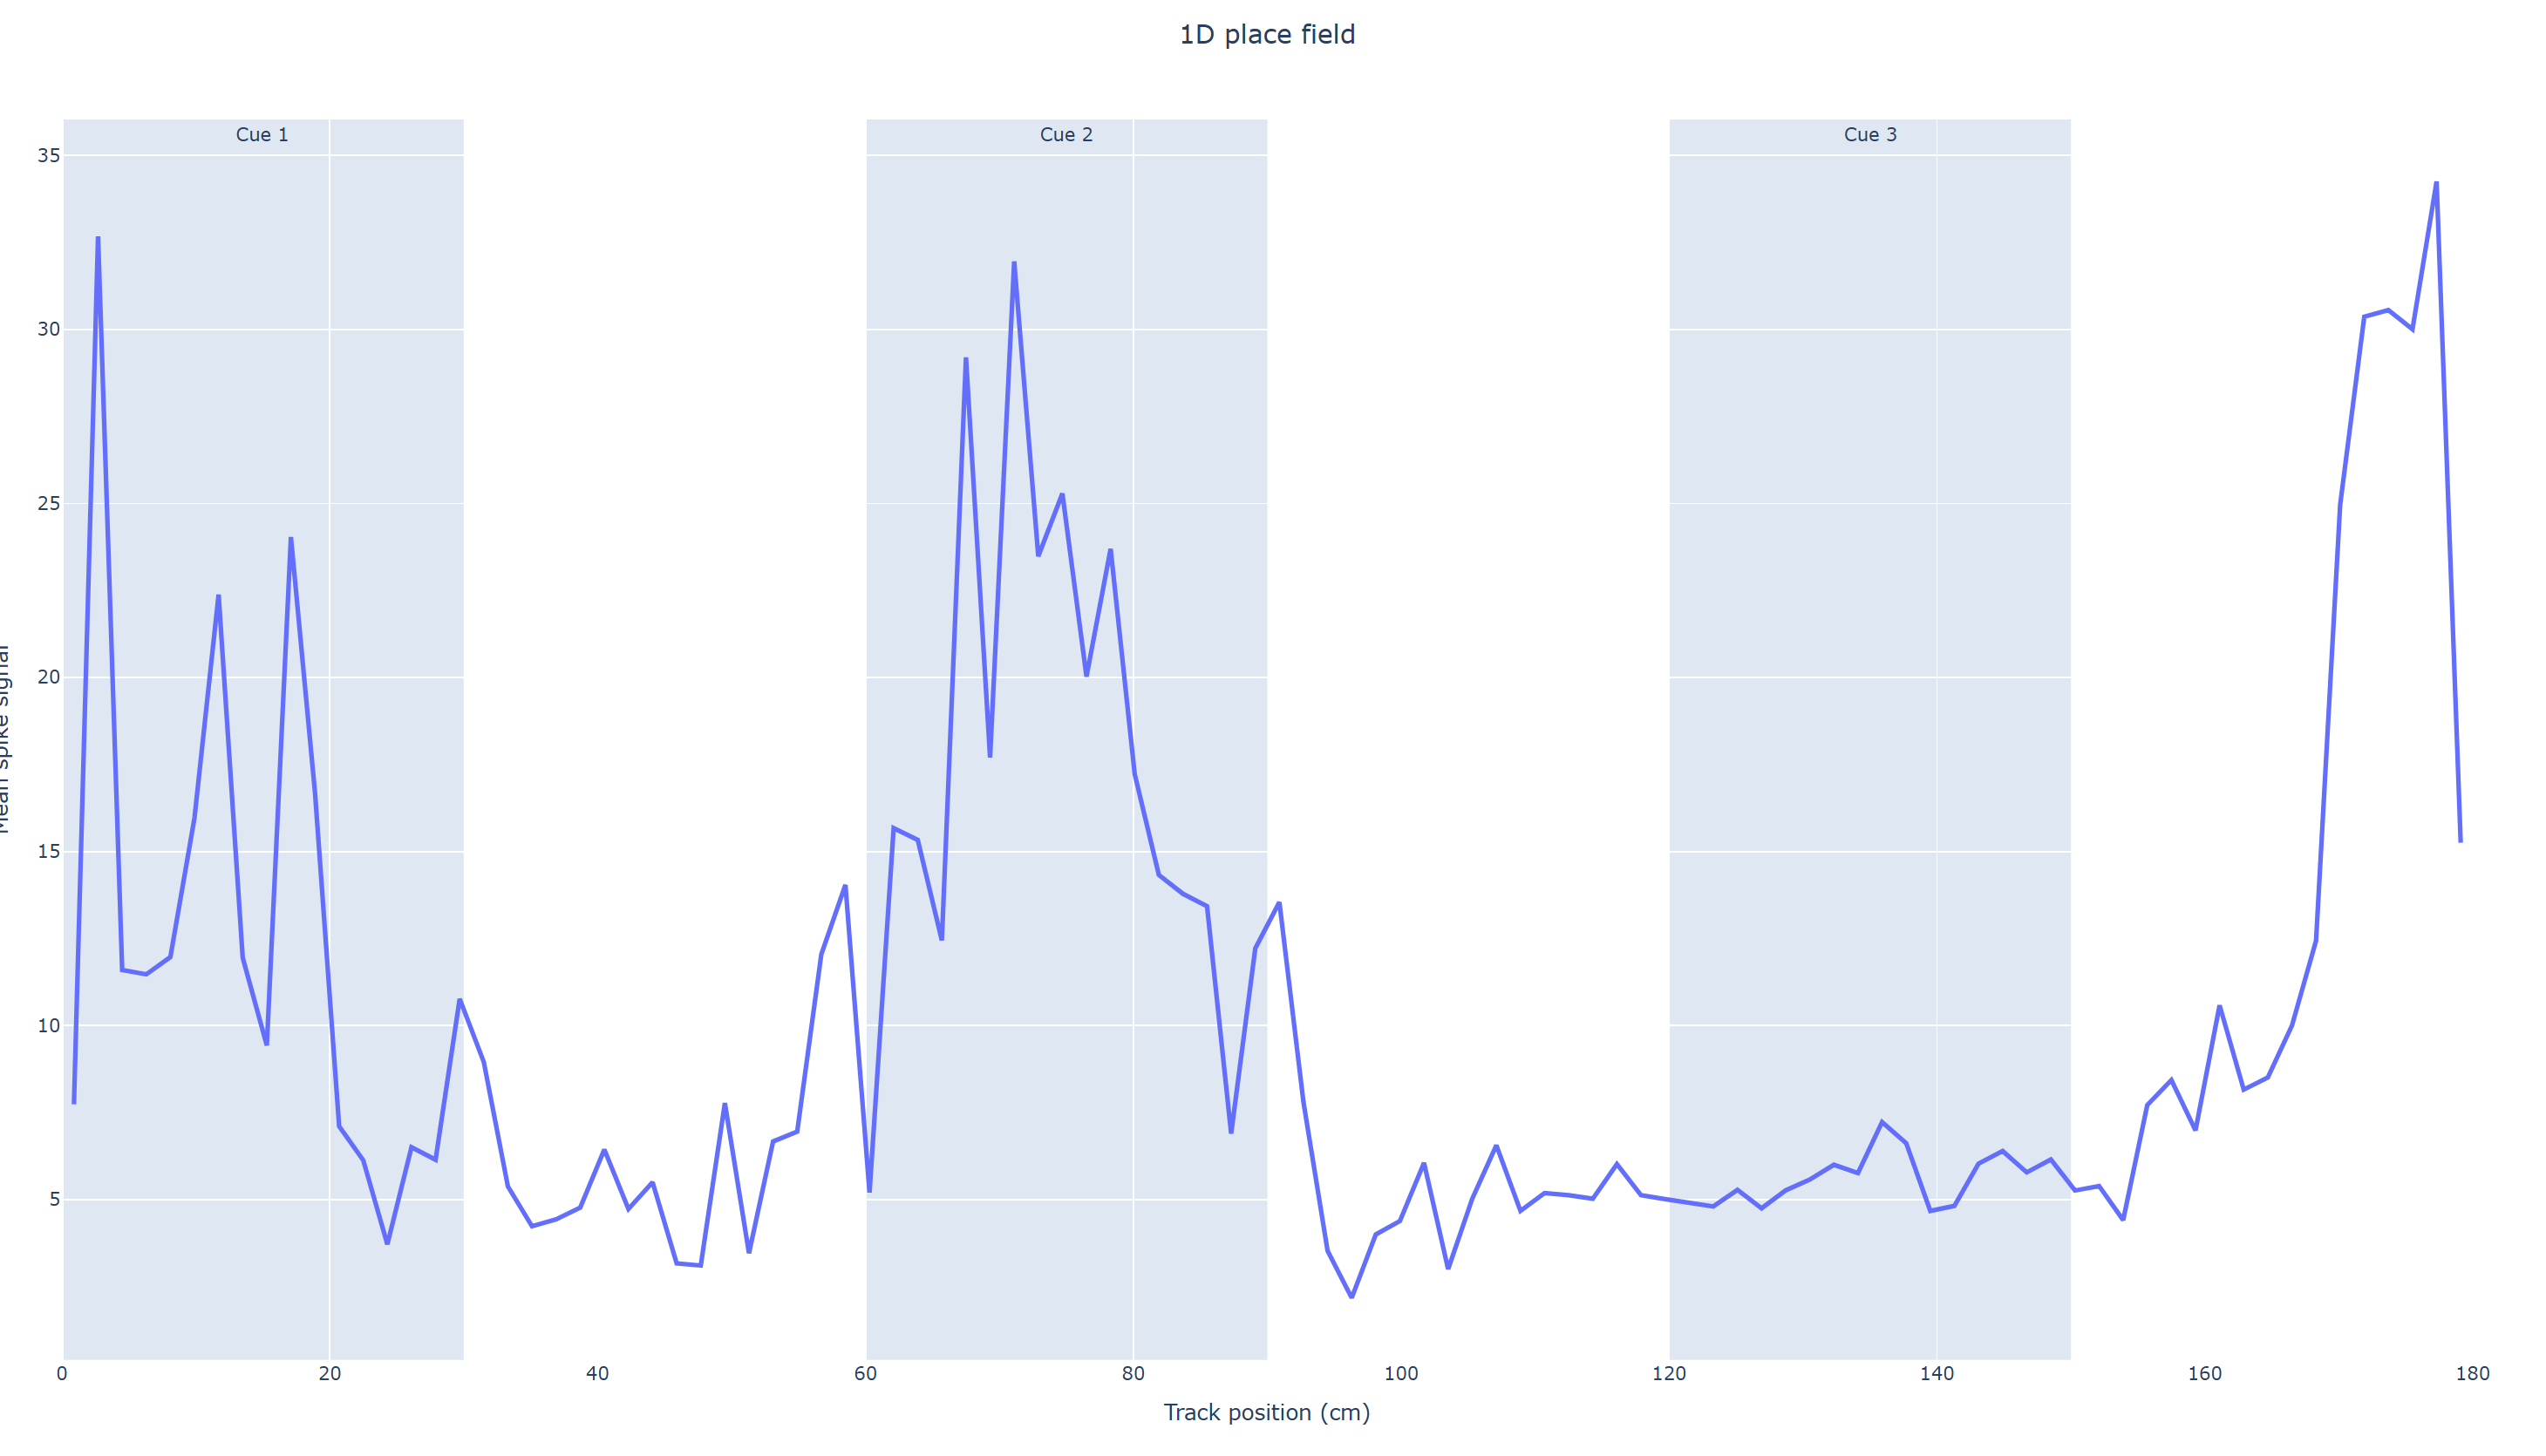
\includegraphics[width=\linewidth]{c2621_day1_rm.png}
\end{minipage}

\vspace{0.02\textwidth}

% -------- Row 2: Day 7 --------
\begin{minipage}[t]{0.48\textwidth}
\vspace{0pt}
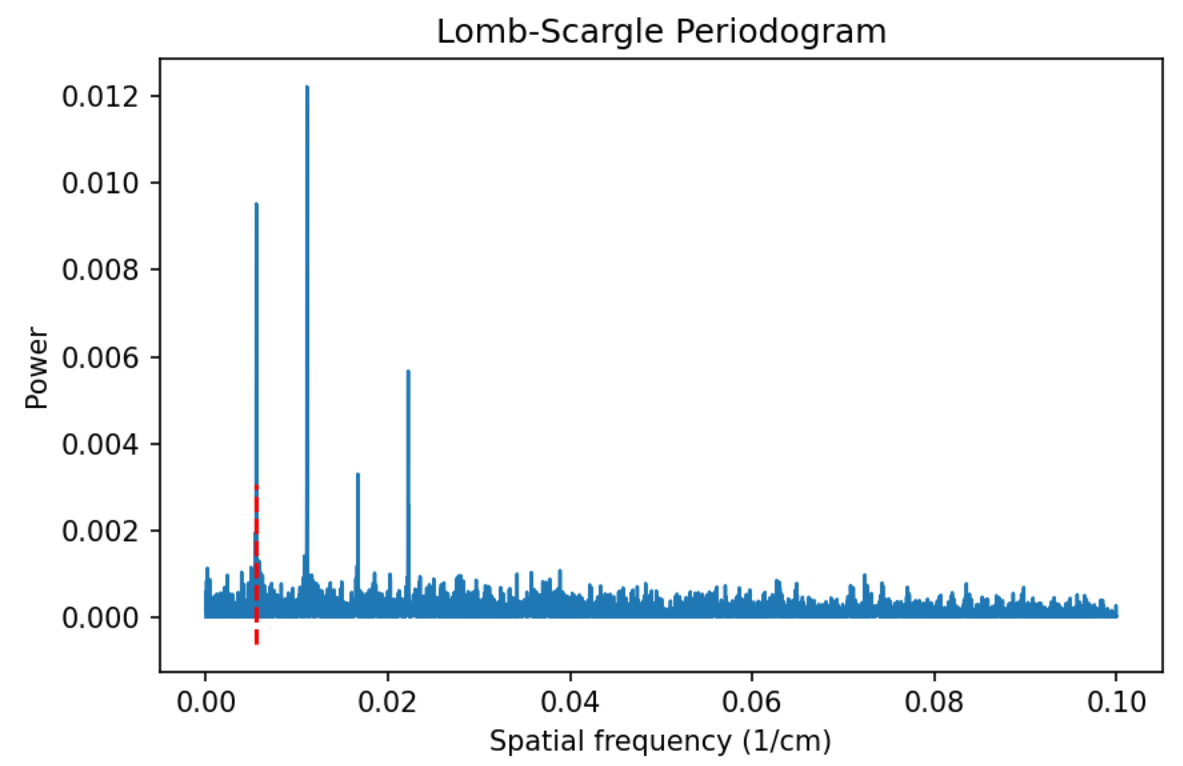
\includegraphics[width=\linewidth]{c2621_day7_per.png}
\end{minipage}\hfill
\begin{minipage}[t]{0.48\textwidth}
\vspace{0pt}
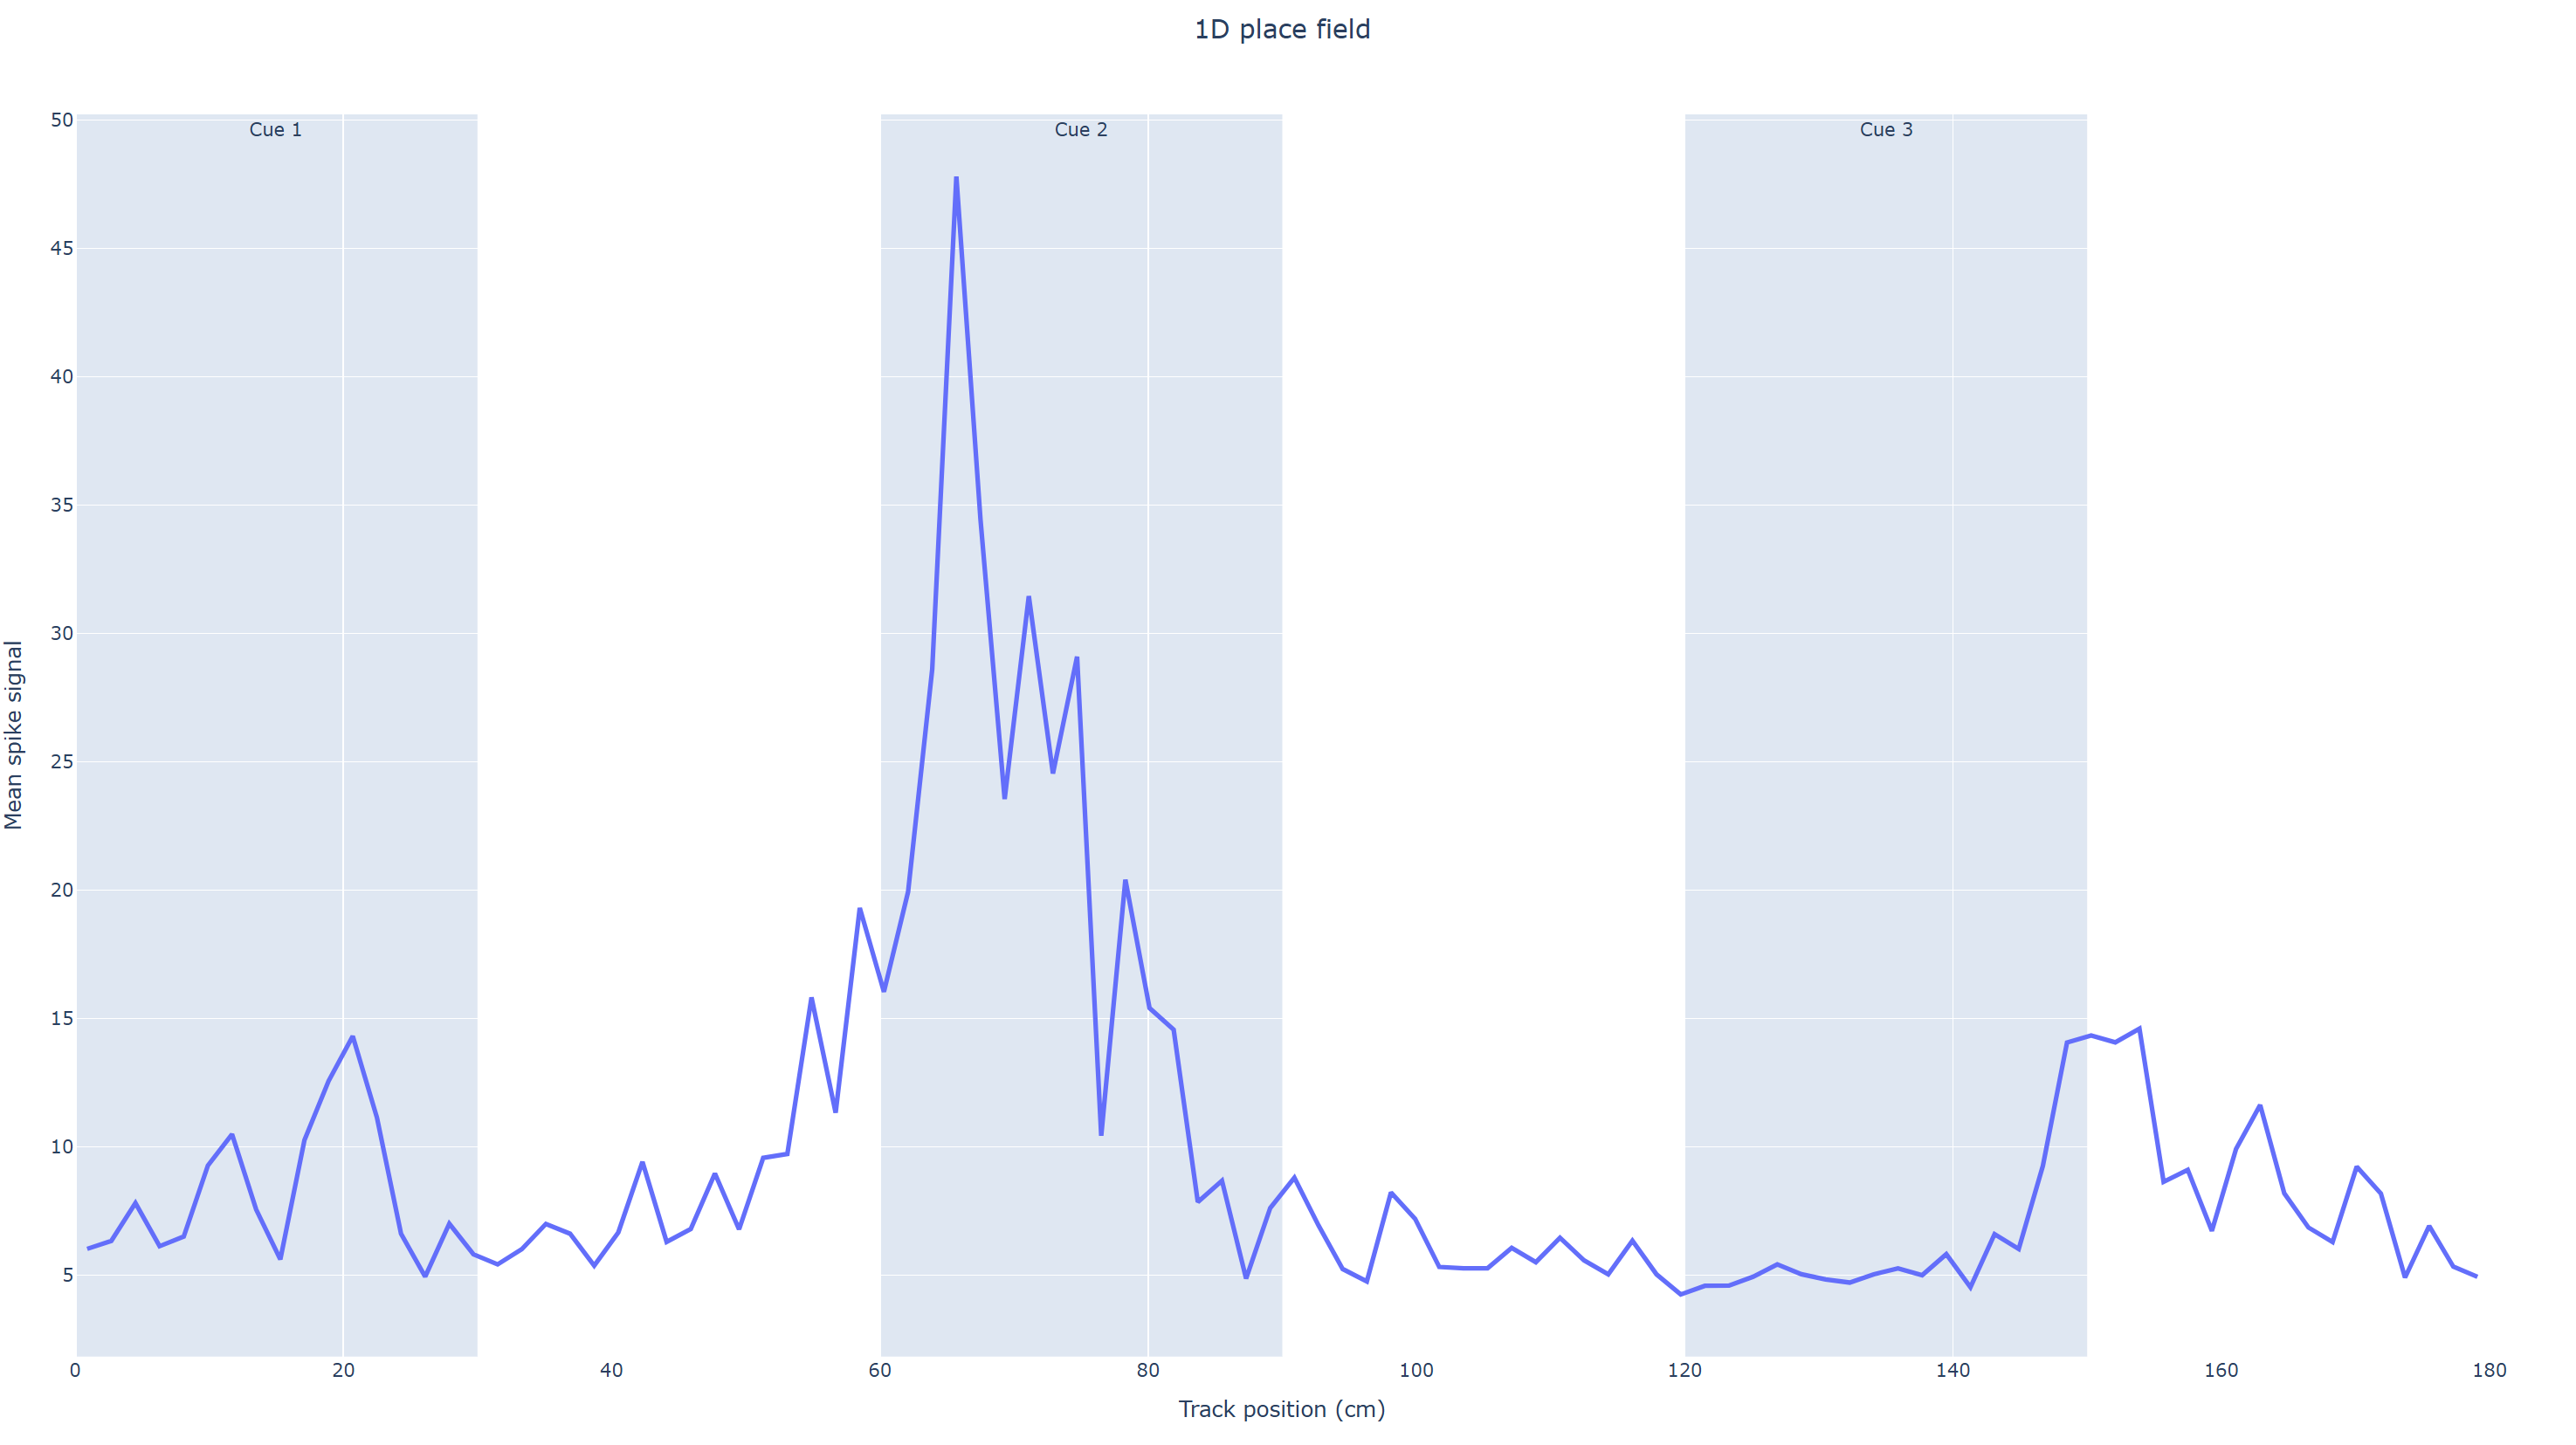
\includegraphics[width=\linewidth]{c2621_day7_rm.png}
\end{minipage}

\vspace{0.02\textwidth}

% -------- Row 3: Day 14 --------
\begin{minipage}[t]{0.48\textwidth}
\vspace{0pt}
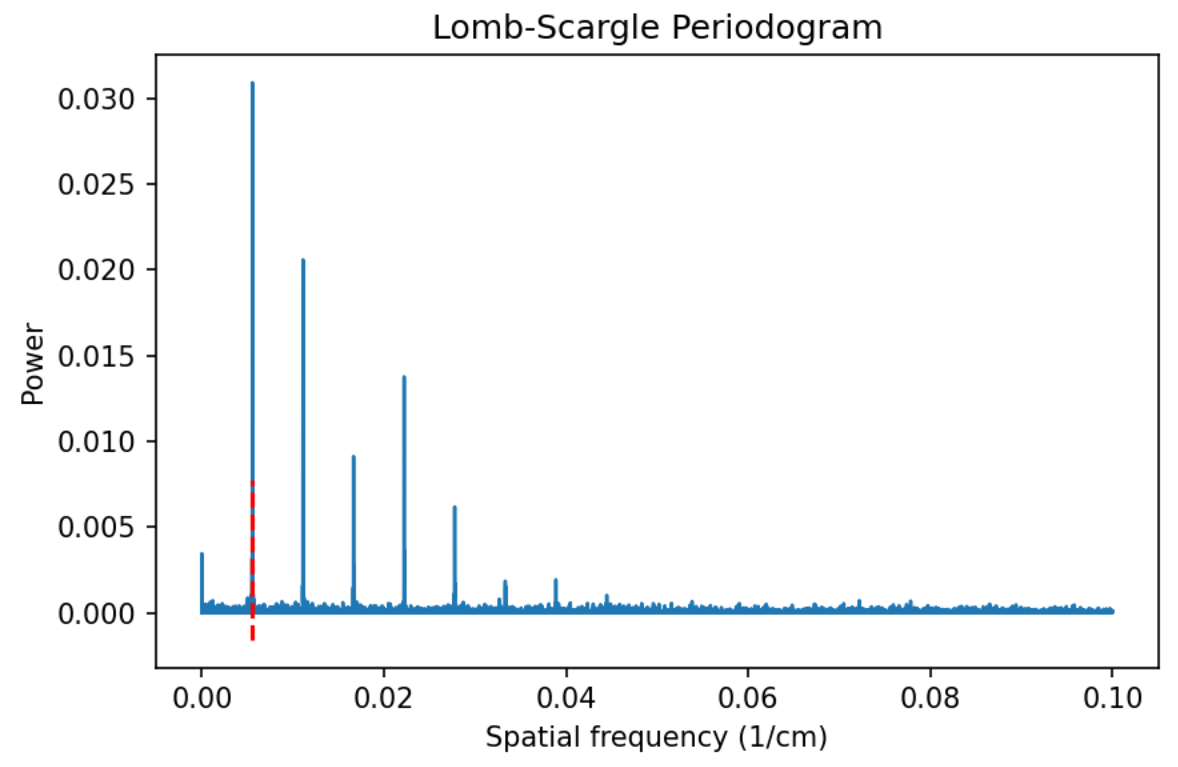
\includegraphics[width=\linewidth]{c2621_day14_per.png}
\end{minipage}\hfill
\begin{minipage}[t]{0.48\textwidth}
\vspace{0pt}
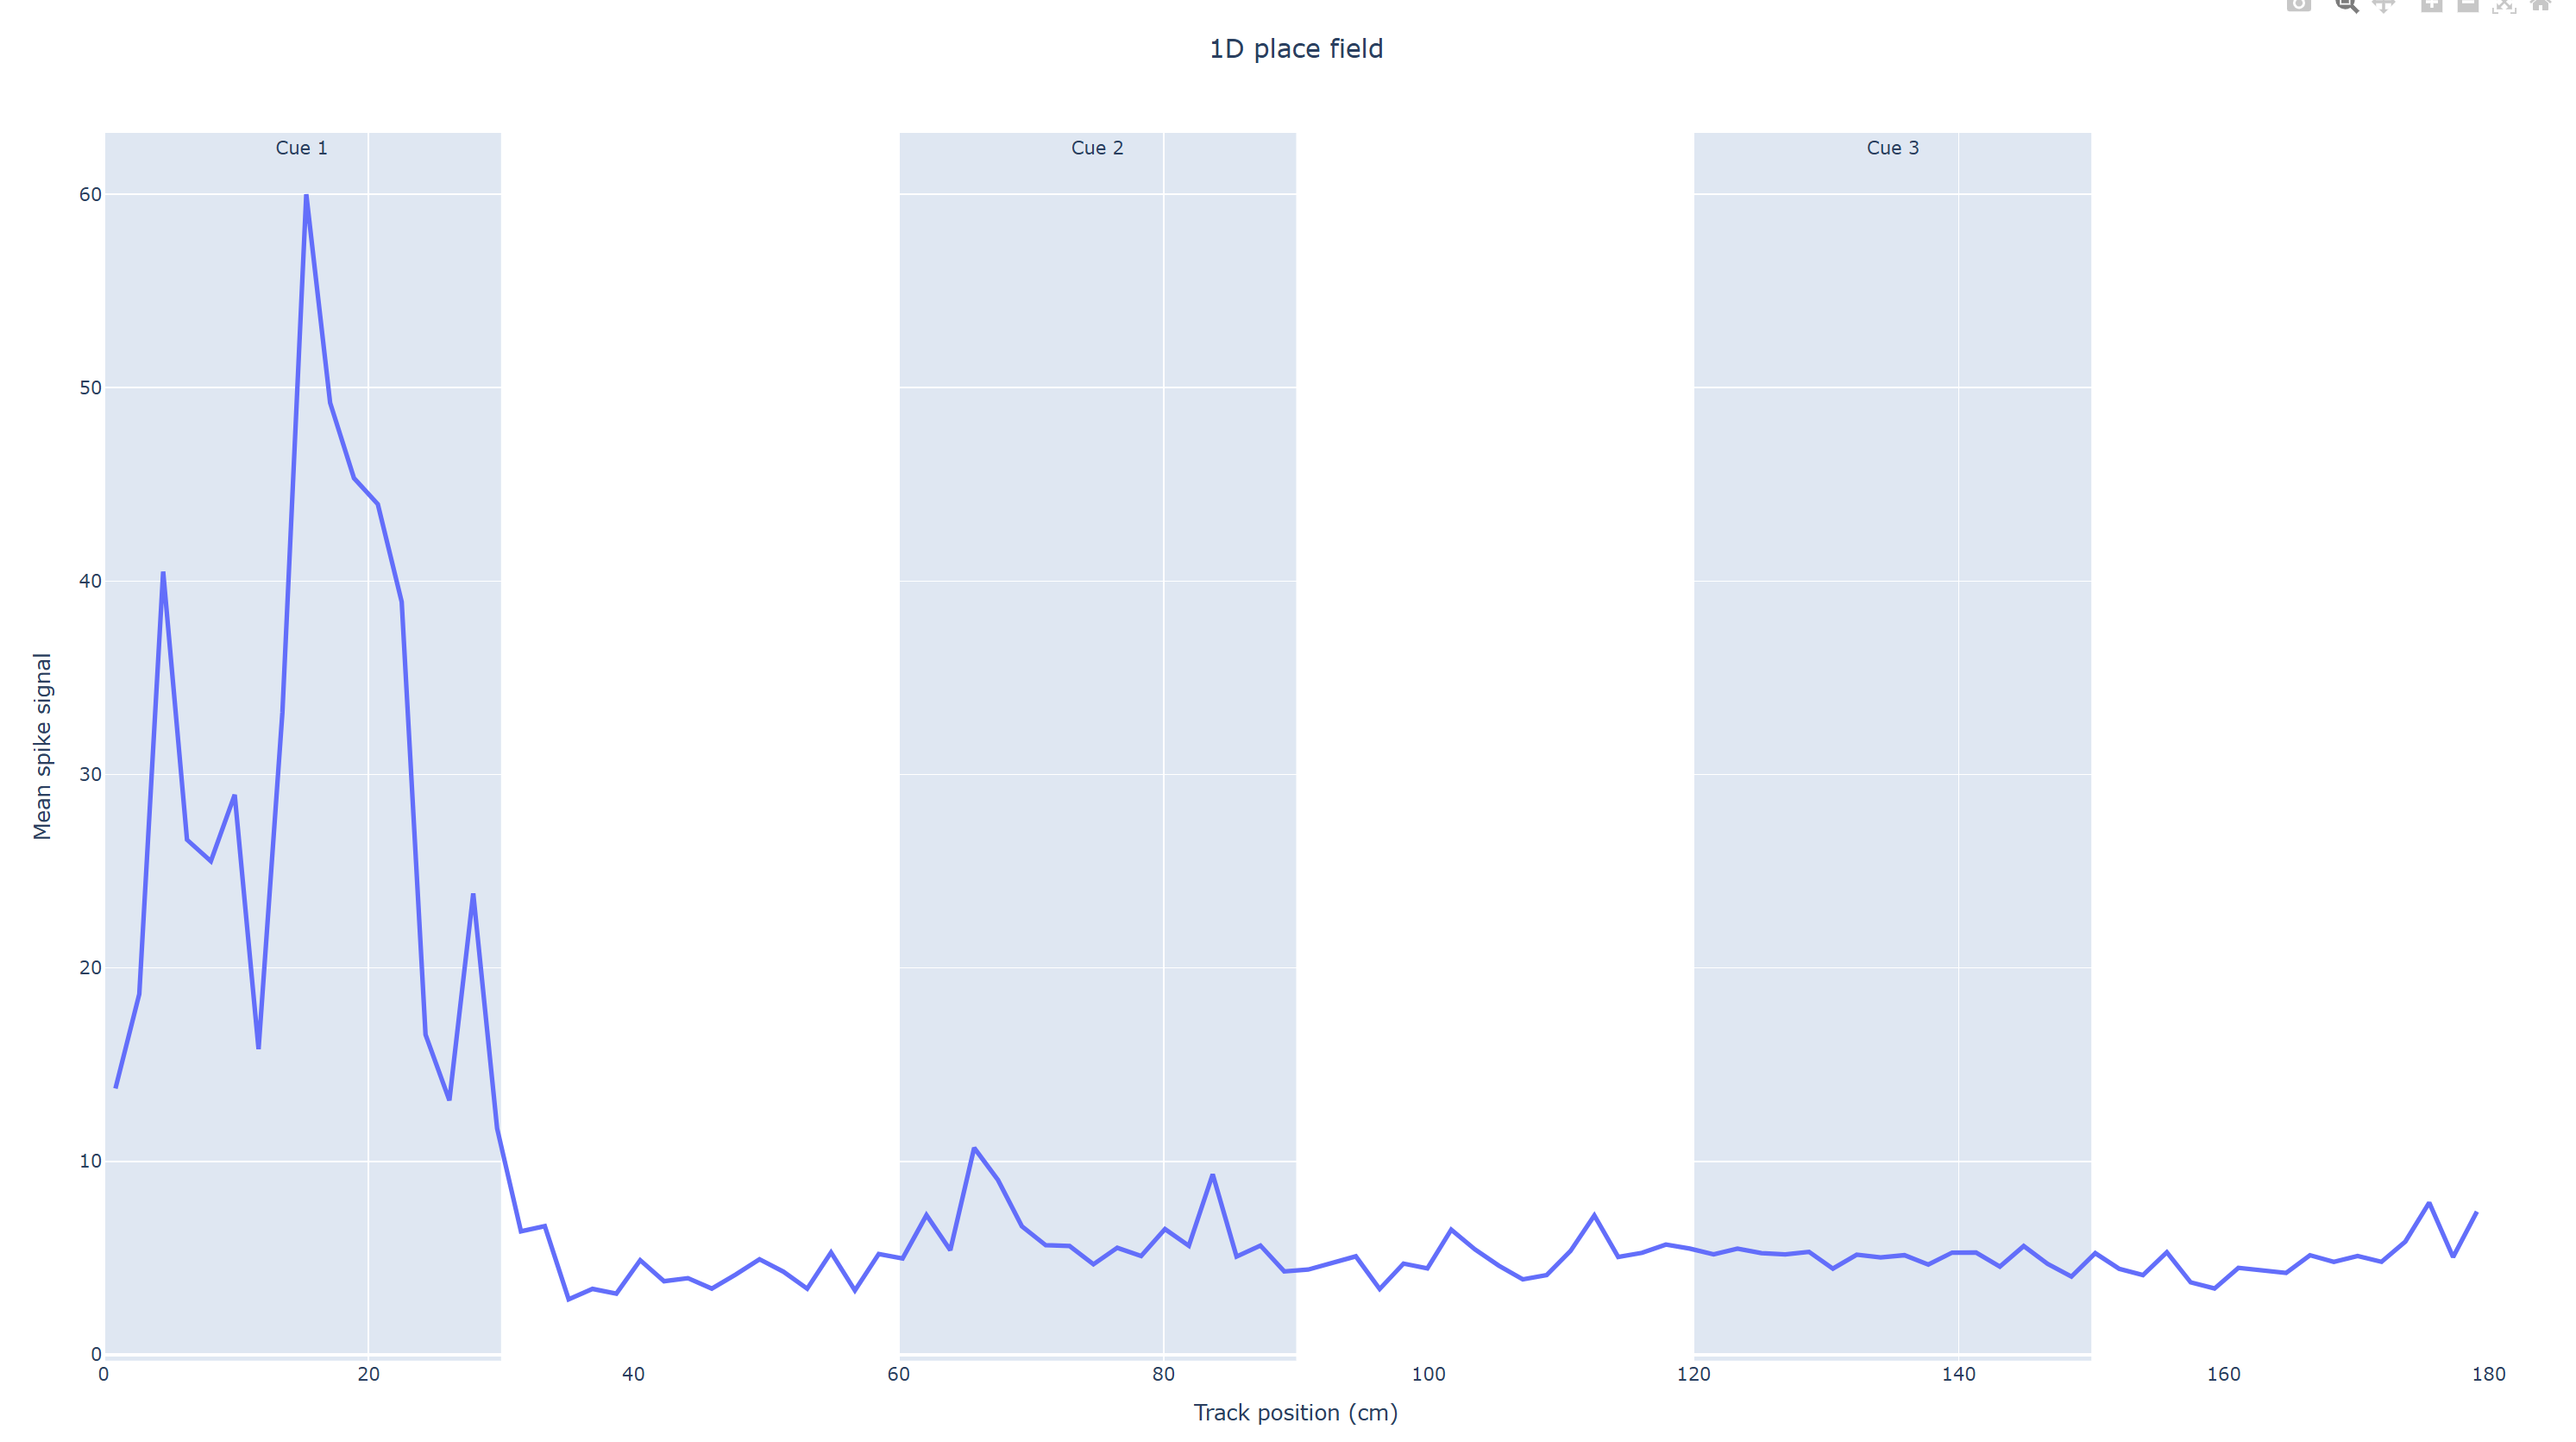
\includegraphics[width=\linewidth]{c2621_day14_rm.png}
\end{minipage}

\caption{
\textbf{Representational drift of a single place cell across sessions.}
(\textit{Left column}) Lomb--Scargle periodograms of Cell~2621 evaluated with respect to position.
(\textit{Right column}) Corresponding spatial rate maps computed using traditional spatial binning.
Rows correspond to recording sessions from the same cell on Day~1 (top), Day~7 (middle), and Day~14 (bottom).
The red dashed line in the periodograms marks the target spatial frequency \(1/180~\mathrm{cm}^{-1}\).
Although the strength of the fundamental spatial frequency increases across sessions, the spatial location of peak firing shifts over time, demonstrating representational drift.
The Lomb--Scargle signal-to-noise ratio (SNR) for this cell increases across sessions:
Day~1: SNR \(= 8.88\),
Day~7: SNR \(= 13.27\),
Day~14: SNR \(= 24.33\).
}
\label{fig:rep_drift_cell2621}
\end{figure}

Next, the cellular activity of individual neurons whose SNR values decreased over time was investigated. The expectation was that as a cell's SNR value increases, its activity becomes more and more concentrated around a single peak while noise decreases. However, the change in activity of a place cell is not so simple. A place cell undergoes representational drift, where the place field shifts location over time. \citep{ziv2013longterm} This is demonstrated by the cell shown in Figure~\ref{fig:rep_drift_cell2621}. On day 1, the periodogram shows high power at multiples of the fundamental frequency \(1/180~\mathrm{cm}^{-1}\). However, the maximum power is actually at 1/60. This is reflected in the day 1 rate map which shows that the cell actually responds when the mouse is near either the first cue or the second cue. It is clear that on day one, the cell activity is quite chaotic, and its low SNR value of 8.88 means that it would not have been characterized as a place cell at this time. However, on day 7, the SNR increases to 13.27 and the place field simplifies. Here, the cell fires only when the mouse is near the second cue. This stabilization is well reflected in the periodogram, as there is a clear increase in the peak of the fundamental frequency \(1/180~\mathrm{cm}^{-1}\), as well as a decrease in harmonics and decrease in the noise. This transition from day 1 to day 7 is the process of recruiting a place cell to track the task structure. When cells that respond to many different parts of the environment become specialized to a single environmental feature (cue 2), the representation of the environment becomes more fine grained, allowing for better performance on the task. 

The transition from day 7 to day 14 shows a second increase in the tuning of this cell to the track structure. This is reflected in a further increase in the power of the fundamental frequency, a further increase in the SNR to 24.33, and a further decrease of the noise. However, when looking at the rate map, something interesting happens. The place field still has a single, distinct peak and zero activity everywhere else, however, this peak has completely changed positions. In this session, the cell responds strongly to cue 1, not cue 2. This is an example of representational drift. Representational drift is a part of the memory consolidation process that is currently not understood by neuroscience experts. The existence of representational drift emphasizes the importance of understanding the behavior of the place cell in context of the network as a whole. To think of these neurons as independent actors misses the fact that all these neurons are highly interconnected and working together. Instead, it is better to think of the brain as a resource allocation strategy which is trying to model its environment. As the mouse recruits more and more place cells to help in understanding the novel environment, the individual cells have their representations reallocated based on network interactions.     
\section{Discussion}

\subsection{Advantage of the Novel Detection Method}
One advantage of using the Lomb--Scargle periodogram as the main detector for place cells is that the periodogram is unaffected by representational drift compared to traditional detection methods which rely on the spatial binning. By converting to the frequency domain, the periodogram and SNR ignores the specifics of what aspect of the environment is being tracked and just measures the degree to which the cell is tracking the environment. This is very useful for longitudinal tracking of place cells over the course of weeks to months, where long term memory consolidation has a major effect on hippocampal place fields. Of course, any analysis of individual cell activity will probably require computing a rate map to actually see where the cell is firing at any given time, but the power spectrum computed by the Lomb--Scargle periodogram serves as a nice complement to these rate maps. The fact that the periodogram can be converted into a single number which reflects the cell's likelihood of being relevant to the task provided a huge time save when manually inspecting cells to assess task learning. 

\subsection{Weakness of the Novel Detection Method}
A key weakness of this method is the reliance on the periodicity in the task structure. In this experiment, the mouse was trained on a simple task of an infinite repeating corridor where each segment was exactly the same as the last. This made for a very clean analysis of spatial frequency. However, many experimental environments studying the hippocampus are much more complicated. For example, consider the same task but where, for each traversal, there is a fifty percent chance of the segment containing an extra cue. All of a sudden, the fundamental frequency is no longer \(1/180~\mathrm{cm}^{-1}\), and the periodogram gets much more difficult to interpret. 

\subsection{Future Directions}

The algorithm executed in this project doesn't actually classify the neurons as a place cell or not a place cell. Instead, it computes a unit-less SNR value which serves as a z-score for how likely the cell is to be a place cell. To further develop this method, it may be beneficial choose a threshold SNR value, so that all cells with SNR higher than the threshold can be classified as a place cell. One way to pick a good threshold would be plotting a histogram of the SNR values considering the distribution. It may be the case that the SNR scores are distributed into two distinct groups, where the cutoff between the groups of SNR scores could be a good candidate threshold. Additionally, knowledge about the distribution of SNR scores could provide some insight into the network dynamics of the hippocampus. 

Another natural direction to take this project is comparison of this method with other place cell methods. It would be great to classify every cell as place cell or no place cell via the SNR's and then classify the same cells using the Peak Method, Stability Method, Information Method, and Combination Method. \citep{grijseels2021choice} This would give a very strong indication of the relevancy of this method. If the majority of identified cells matched across different detection methods, then this would suggest robustness of the novel method. On the other hand, cells which were classified differently by different methods would provide insight on how to improve this method as well as possible  weaknesses in traditional methods due to reliance on spatial binning.

While this project focuses solely on the power spectrum with respect to spatial frequencies, there may be additional insight to gain by also analyzing the temporal power spectrum of the data. Hippocampal neurons exhibit prominent oscillatory dynamics across multiple temporal scales, most notably in the theta (4--10 Hz) and gamma (30--100 Hz) bands. These oscillations are thought to play a critical role in coordinating neural activity during spatial navigation and memory formation. For example, place cell firing is strongly modulated by the phase of the theta rhythm, a phenomenon known as theta phase precession, in which spikes occur at progressively earlier phases of the theta cycle as the animal traverses a place field \citep{okeefe1993phase}. Combining spatial-frequency analysis with temporal spectral analysis could therefore provide a richer description of hippocampal representations. Cells that exhibit strong spatial periodicity may differ in how their activity is temporally organized, potentially reflecting distinct functional roles within the hippocampal network. Joint spatiotemporal spectral analyses may help disentangle cells that encode spatial position from those that primarily reflect internal network dynamics or behavioral state, offering a more comprehensive framework for place cell classification and hippocampal population analysis.


\section{Code Availability}
All analysis code used in this study, including Lomb--Scargle periodogram computation, signal-to-noise ratio (SNR) scoring, and spatial rate-map generation, is publicly available on GitHub at \url{https://github.com/Jgroner11/Hippo-Fourier}. The experimental data are proprietary and therefore not included in the repository; however, the \texttt{results} directory contains summary statistics as well as representative Lomb--Scargle periodograms and spatial rate maps for individual cells, organized by SNR.

\bibliographystyle{aasjournalv7}
\bibliography{references}



\end{document}
